
\chapter{Recherche d'une violation de la symétrie de Lorentz avec CMS au LHC} \label{chap:chap5}

\begin{fmffile}{chapitre5}


La dernière et principale étude présentée dans cette thèse est la recherche de la violation de la symétrie de Lorentz dans le secteur du quark $\Ptop$. Plus précisément, l'analyse cherche à mesurer le processus suivant en fonction du temps sidéral avec les données de CMS au LHC :
\begin{equation}
\ttbar \rightarrow \Pbottom \Pleptonplus \Pnulepton +  \APbottom \Pleptonminus \APnulepton
\end{equation}
avec les couples de leptons $(\Pleptonplus,\Pleptonminus) = (\APelectron, \Pmuon)$ ou $(\Pleptonplus,\Pleptonminus) = (\APmuon, \Pelectron)$. Ce processus est le canal dilepton du processus $\ttbar$ (présenté dans la section \ref{sec:quarktop}). L'analyse se focalise sur les données de 2016 et 2017,  qui fournissent une luminosité de respectivement $\mathcal{L}^\textrm{2016} = \SI{35.9}{\femto \barn^{-1}}$ et $\mathcal{L}^\textrm{2017} = \SI{41.5}{\femto \barn^{-1}}$, soit une luminosité intégrée totale de $\mathcal{L} = \SI{77.4}{\femto \barn^{-1}}$. Les données acquises en 2018, ainsi que les simulations qui les accompagnent, n'étaient pas disponibles lorsque j'ai commencé l'analyse et ne sont pas utilisées dans cette thèse.

On a montré dans le chapitre \ref{chap:chap2} que la violation de Lorentz dans ce secteur fournit un signal caractéristique : une oscillation de la section efficace de la production \ttbar au cours du temps sidéral. Pour mesurer cette oscillation, on utilisera comme observable discriminante la masse dilepton (présentée dans la section \ref{mdilep}) qui présente un bon pouvoir de discrimination entre signal et bruits de fond.
La stratégie consiste à faire une comparaison entre la distribution de la masse dilepton dans le cas du Modèle Standard (distribution obtenue par simulation) et celle mesurée dans les données en fonction du temps sidéral, puis d'en extraire une valeur des coefficients $c_{\mu\nu}$ par analyse statistique.

Cette recherche se découpe en deux temps. Premièrement, il faut à partir de fichiers d'évènements bruts (données mesurées et simulations Monte-Carlo) fournis par la collaboration, faire une sélection des évènements intéressants. Cette étape, appelée chaîne d'analyse, est gérée par un logiciel développé par l'équipe CMS du CERN et utilisé à l'IP2I \cite{heppy} codé en langage \texttt{C++} et \texttt{Python}. 
Après validation de la chaîne d'analyse, une étude statistique est produite pour extraire le signal. Il s'agit d'utiliser une méthode d'ajustement par maximum de vraisemblance. Cette procédure est réalisée à l'aide de l'outil de la collaboration CMS \cite{combine}. Les dernières mises à jour de l'analyse sont disponible dans l'\emph{Analysis Note} \cite{ANnous}.

\section{Reconstruction des évènements et identification des objets}

Au niveau du détecteur, le processus dilepton engendre des évènements dont les produits détectables sont de type électron, muon et quark $\Pbottom$ (voir figure \figurename{\ref{fig:temoin}}). 

\begin{figure}[h]
\begin{center}
        \vspace{0.5cm}
        \begin{fmfgraph*}(180,150)
                \fmfpen{0.5}
                \fmfleft{t1,i1,i2,t2}
                \fmfright{o1,o2,o3,o4,o5,o6}
        
                \fmf{gluon}{i1,v1,i2}   
                \fmf{gluon}{v1,v2}
                \fmf{fermion,label=\APtop,label.side=left}{v3,v2}
                \fmf{fermion,label=\Ptop,label.side=left}{v2,v4}
                \fmf{boson,label=\PWplus,label.side=left}{v4,v6}
                \fmf{boson,label=\PWminus,label.side=right}{v3,v5}
                \fmf{fermion, foreground=blue}{v5,o1}
                \fmf{fermion, foreground=blue}{o6,v6}
        
                \fmffreeze
        
                \fmf{fermion, foreground=red}{o3,v3}
                \fmf{fermion, foreground=red}{v4,o4}
        
                \fmf{fermion}{v6,o5}
                \fmf{fermion}{o2,v5}
        
                \fmflabel{\textcolor{blue}{\Pleptonminus}}{o1}
                \fmflabel{\APnulepton}{o2}
        
                \fmflabel{\textcolor{red}{\APbottom}}{o3}
                \fmflabel{\textcolor{red}{\Pbottom}}{o4}
        
                \fmflabel{\Pnulepton}{o5}
                \fmflabel{\textcolor{blue}{\Pleptonplus}}{o6}
        
                \fmfdot{v1,v2,v3,v4,v5,v6}
            \end{fmfgraph*}
            \vspace{0.5cm}
    \caption{Diagramme de Feynman du processus $\ttbar$ dans le canal dilepton. Les produits caractéristiques de ce canal portent les couleurs bleue pour les leptons et rouge pour les quarks $\Pbottom$.}
    \label{fig:temoin}
\end{center}
\end{figure}

Pour discriminer le signal des autres processus de bruits de fond du Modèle Standard, une sélection sur les évènements est opérée. Cette sélection est présentée dans la section suivante. Cependant, malgré la sélection, certains processus produisent dans le détecteur un état final qui ressemble trop au signal et passent les critères de sélection. Il faut les prendre en compte et les soustraire à l'aide d'une analyse statistique. Une liste exhaustive des bruits de fond ainsi que leurs description est présentée dans la section suivante. 



\section{Sélection des évènements}

Pour sélectionner les évènements, la première étape est de ne retenir que ceux qui ont satisfaits les critères du système de déclenchement de haut niveau. Cette pré-sélection est dite "en ligne" (ou \emph{online}). Après l'acquisition par le détecteur, on peut raffiner les critères en appliquant \emph{a posteriori} une sélection plus forte. Il s'agit d'une sélection "hors-ligne" (ou \emph{offline}). Ces deux sélections sont présentées dans les paragraphes suivant. 


\subsection{Sélection sur les chemins de déclenchement}

\begin{sloppypar}
La pré-sélection, tant pour l'année 2016 que 2017, contient des critères sur l'impulsion transverse minimale, la pseudo-rapidité, l'isolation et la compatibilité des traces avec le vertex primaire. On ne montre ici que les évènements qui passent des critères d'impulsions transverses minimales. Ces critères sont distincts dans le cas de déclencheurs de types double leptons (déclencheurs \Pe{}\Pmu{} dans cette analyse) et les déclencheurs de types lepton seul. Le résumé de ces critères se trouve dans les tableaux \tablename{\ref{fig:trig}}.
Il est à noter que ces chemins de déclenchement de haut niveau s'appliquent par dessus des critères de déclenchement de niveau 1 moins restrictifs. L'ensemble des événements satisfaisant les critères de niveau 1 sont compris dans un lot de données appelé "lot de données premier" (\emph{primary dataset}), qui est celui sur lequel le code d'analyse s'applique. Ces mêmes critères sont inclus dans les échantillons de simulation.

\end{sloppypar}

\begin{table}
\begin{subtable}[b]{0.5\textwidth}
\begin{tabular}{c|cc}
    \noalign{\smallskip}\hline\noalign{\smallskip}
    \multirow{2}{*}{Déclenchement} &\multicolumn{2}{r}{\pt minimum requis} \\
    &\Pmu & \Pe\\
    \noalign{\smallskip}
    \hline \hline
    \noalign{\smallskip}
    \multirow{2}{*}{double lepton}&\SI{23}{\GeV} & \SI{12}{\GeV} \\
    &\SI{8}{\GeV} & \SI{23}{\GeV} \\    
    \noalign{\smallskip}\hline\noalign{\smallskip}
    \multirow{2}{*}{lepton seul}&\SI{24}{\GeV} & \\
    && \SI{27}{\GeV} \\
    \noalign{\smallskip}\hline\noalign{\smallskip}
\end{tabular}
\caption{2016}
\label{fig:trig2016}
\end{subtable}
\begin{subtable}[b]{0.5\textwidth}
\begin{tabular}{c|cc}
    \noalign{\smallskip}\hline\noalign{\smallskip}
    \multirow{2}{*}{Déclenchement} &\multicolumn{2}{r}{\pt minimum requis} \\
    &\Pmu & \Pe\\
    \noalign{\smallskip}
    \hline \hline
    \noalign{\smallskip}
    \multirow{2}{*}{double lepton}&\SI{23}{\GeV} & \SI{12}{\GeV} \\
    &\SI{8}{\GeV} & \SI{23}{\GeV} \\    
    \noalign{\smallskip}\hline\noalign{\smallskip}
    \multirow{2}{*}{lepton seul}&\SI{27}{\GeV} & \\
    && \SI{35}{\GeV} \\
    \noalign{\smallskip}\hline\noalign{\smallskip}
\end{tabular}
\caption{2017}
\label{fig:trig2017}
\end{subtable}
\caption{Liste des critères de déclenchement de haut niveau utilisées dans cette analyse pour les années (\subref{fig:trig2016}) 2016 et (\subref{fig:trig2017}) 2017, appliqués dans les données et la simulation.}
\label{fig:trig}
\end{table}

L'ensemble exhaustif des chemins de déclenchement de haut niveau utilisés dans l'analyse est donné dans l'annexe \ref{HLTpath}.

\subsection{Sélection hors-ligne}\label{btagref}

La première étape de la sélection consiste à ne garder que des évènements comportant un seul couple de leptons avec un électron et un muon. Pour cela, l'évènement est retenu si les deux leptons respectent un $\Delta R(\Pe{},\Pmu{}) > \num{0.5}$ pour éviter les chevauchements. Il doivent aussi avoir des charges électriques de signe opposé. Ensuite l'évènement retenu doit avoir au moins deux jets reconstruits de $\pt > \SI{30}{\GeV}$ et $|\eta|<\num{2.4}$, et parmi eux au moins au moins un jet étiqueté \Pbottom.
\newline

Plus précisément, chaque particule est soumise à des critères de sélection dont certains sont présentés au chapitre précédent (chapitre \ref{chap:chap4}). Pour les leptons, celui de plus haut $\pt$ nommé dominant (ou \emph{lead}) est sélectionné différemment du second lepton (\emph{sublead}). Pour plus de précisions voir le tableau \tablename{\ref{table:critlepton}}.
\begin{table}
\begin{center}
\begin{tabular}{ccc}
    \noalign{\smallskip}\hline\noalign{\smallskip}
    Critères & Muon & Électron \\
    \noalign{\smallskip}
    \hline \hline
    \noalign{\smallskip}
    $\pt^\textrm{\emph{lead}}$ minimum  & \SI{25}{\GeV} & \SI{25}{\GeV} \\
    $\pt^\textrm{\emph{sublead}}$ minimum & \SI{20}{\GeV} & \SI{20}{\GeV} \\
    $|\eta|$   maximum & \num{2.4} & \num{2.4}  (écart EB/EE exclu\footnotemark)\\
    Identification \emph{particle-flow} & tight & tight \\
    Isolation \emph{particle-flow} & tight & tight \\
    \noalign{\smallskip}\hline\noalign{\smallskip}
\end{tabular}
\end{center}
\caption{Critères de sélection hors-ligne appliqués aux leptons.}
\label{table:critlepton}
\end{table}
\footnotetext{Dans le ECAL, l'écart entre le tonneau (EB) et le bouchon (EE) est exempt de zone de détection, on le retire donc pour la sélection.}

Pour les jets, il est demandé que chaque évènement en comporte au moins deux dont un étiqueté \Pbottom. De plus, il est demandé aux jets de répondre à une contrainte supplémentaire : la fraction en lepton du jet doit être inférieure à \num{0.80}. On dit que ces jets passent le critère \emph{tight + veto lepton} (voir figure \figurename{\ref{table:critjet}}). Une correction à l'énergie des jets fournie par la collaboration est appliquée.
\begin{table}
\begin{center}
\begin{tabular}{cc}
    \noalign{\smallskip}\hline\noalign{\smallskip}
    Critères & Jets  \\
    \noalign{\smallskip}
    \hline \hline
    \noalign{\smallskip}
    $\pt$ minimum  & \SI{30}{\GeV} \\
    $|\eta|$   maximum & \num{2.4}\\
    Identification \emph{particle-flow} & tight + veto lepton\\
    $\Delta R (\textrm{jet,lepton})$ minimum & \num{0.4} \\
    \noalign{\smallskip}\hline\noalign{\smallskip}
\end{tabular}
\end{center}
\caption{Critères de sélection hors-ligne appliqués aux jets.}
\label{table:critjet}
\end{table}
 Pour l'étiquetage des jets \Pbottom, on utilise l'algorithme \emph{DeepCSV} (présenté dans la section \ref{sec:b_tagging} du chapitre précédent) avec un critère lâche (\emph{loose working point}). Ce critère demande une valeur de coupure de 0.2217 pour l'année 2016 et 0.1522 pour l'année 2017.

\subsection{Reconstruction de la masse dilepton}\label{mdilep}

La masse dilepton est une variable discriminante à partir de laquelle seront extraits les résultats. Elle est préférée à la masse transverse car l'utilisation de l'énergie transverse manquante dégraderait la discrimination signal sur bruit. En revanche, la masse dilepton est la meilleure variable car elle ne fait intervenir que des observables leptoniques donc bien mesurées.
Elle est définie comme :
\begin{align}
    m^2_{\Pleptonminus \Pleptonplus} &= \left\| p_{\Pleptonminus} + p_{\Pleptonplus}   \right\|^2 \nonumber \\
    &= m_{\Pleptonminus}^2 + m_{\Pleptonplus}^2 + 2 (E_{\Pleptonminus} E_{\Pleptonplus} - \vec{p}_{\Pleptonminus} \cdot \vec{p}_{\Pleptonplus})
\end{align}
où les $p_i$ représentent les 4-impulsions des produits de désintégration dileptonique de la paire \ttbar.

\section{Les bruits de fond}

Malgré la sélection, d'autres processus du Modèle Standard sont toujours présents, ils sont appelés bruit de fond.
Quelques diagrammes représentatifs de ces bruits de fond sont visibles sur la figure  \figurename{\ref{fig:background}}. Une liste des échantillons utilisés dans l'analyse est présentée sous forme d'équation de réaction avec les sections efficaces associées dans la table \tablename{\ref{tab:MC}}.


\begin{figure}
    \centering
    \subcaptionbox{\label{fig:bkg1}}[0.48\textwidth]{
   \begin{fmfgraph*}(180,150)
           \fmfpen{0.5}
           \fmfleft{i1,i2}
           \fmfright{o1,o2,o3,o4}

           \fmf{fermion}{i1,v1,v2,i2}
           \fmf{boson,label=\PWminus,label.side=left}{v1,v3}
           \fmf{boson,label=\PWplus,label.side=right}{v2,v4}
   
          \fmflabel{\Pquark}{i1}
          \fmflabel{\APquark}{i2}
   
           \fmf{fermion}{o1,v3}
           \fmf{fermion}{v3,o2}
   
           \fmf{fermion}{v4,o3}
           \fmf{fermion}{o4,v4}
   
           \fmflabel{\Pleptonminus}{o1}
           \fmflabel{\APnulepton}{o2}

           \fmflabel{\Pnulepton}{o3}
           \fmflabel{\Pleptonplus}{o4}
   
           \fmfdot{v1,v2,v3,v4}
       \end{fmfgraph*}}\hfill
    \subcaptionbox{\label{fig:bkg3}}[0.48\textwidth]{
   \begin{fmfgraph*}(180,150)
           \fmfpen{0.5}
           \fmfleft{i1,i2}
           \fmfright{o1,o2,o3,o4}

           \fmf{fermion}{i2,v2,v1}
           \fmf{gluon}{i1,v1}
           \fmf{fermion,label=$\Pquark^\prime$,label.side=left}{v1,v3}
           \fmf{boson,label=\PWminus,label.side=right}{v2,v4}
   
            \fmflabel{\Pquark}{i2}
   
           \fmf{fermion}{v3,o1}
           \fmf{fermion}{v3,o2}
   
           \fmf{gluon}{v4,o3}
           \fmf{fermion}{v4,o4}
   
           \fmflabel{jet}{o1}
           \fmflabel{jet}{o2}

           \fmflabel{\APnulepton}{o3}
           \fmflabel{\Pleptonminus}{o4}
           
            \fmfblob{.12w}{v3}
           \fmfdot{v1,v2,v4}
       \end{fmfgraph*}}
       \\\vspace{0.5cm}
    \subcaptionbox{\label{fig:bkg2}}[0.48\textwidth]{
    \begin{fmfgraph*}(180,150)
            \fmfpen{0.5}
            \fmfleft{t1,i1,i2,t2}
            \fmfright{o1,o2,o3,o4,o5,o6}
    
            \fmf{gluon}{i1,v1}
            \fmf{fermion}{i2,v1}
            \fmf{fermion}{v1,v2}
            \fmf{phantom}{v3,v2}
            \fmf{fermion,label=\Ptop,label.side=left}{v2,v4}
            \fmf{boson,label=\PWplus,label.side=left}{v4,v6}
            \fmf{phantom}{v3,v5}
            \fmf{fermion}{v5,o1}
            \fmf{fermion}{o6,v6}
    
            \fmffreeze
            
            \fmf{boson,label=\PWminus,label.side=right}{v2,v5}
            \fmf{phantom}{o3,v3}
            \fmf{fermion}{v4,o4}
    
            \fmf{fermion}{v6,o5}
            \fmf{fermion}{o2,v5}
    
            \fmflabel{\Pbottom}{i2}
            \fmflabel{\Pleptonminus}{o1}
            \fmflabel{\APnulepton}{o2}
    

            \fmflabel{\Pbottom}{o4}
    
            \fmflabel{\Pnulepton}{o5}
            \fmflabel{\Pleptonplus}{o6}
    
            \fmfdot{v1,v2,v4,v5,v6}
        \end{fmfgraph*}}
    \caption{Diagrammes de Feynman des processus de bruit de fond de (\subref{fig:bkg1}) $\PW{}\PW$,  (\subref{fig:bkg3}) $\PW{}$ + jets et (\subref{fig:bkg2}) top solitaire dans le canal \Ptop{}\PW{}.}
    \label{fig:background}
\end{figure}


\begin{description}
\item[Quark top solitaire]
\begin{sloppypar}
Il s'agit du bruit de fond principal. Il est particulièrement représenté car la présence d'un quark $\Ptop$ (respectivement $\APtop$) engendrera un quark $\Pbottom$ (respectivement $\APbottom$) étiqueté avec l'algorithme DeepCSV (voir section \ref{sec:b_tagging}). Il y a trois processus de top solitaire : $t$-channel, \Ptop{}\PW{} et $s$-channel déjà présentés dans la section \ref{sec:quarktop} du chapitre \ref{chap:chap2}. Le principal processus après sélection est le \Ptop{}\PW{}, en raison de la presence du \Ptop  et du boson \PW qui peuvent donner chacun un lepton.
\end{sloppypar}
\item[Processus top-antitop + $X$ (ou $ttX$)]
\begin{sloppypar}
Ces processus sont explicitement parasites car ils produisent le même état final que \ttbar. Ils portent en plus les produits de désintégration de la particule $X$ qui est soit un \PWpm soit un \PZ.
\end{sloppypar}
\item[Dibosons]
\begin{sloppypar}
La production de paires de bosons vecteurs (\PW{}\PW{}, \PW{}\PZ{}, \PZ{}\PZ{}) peut représenter une source de bruit de fond non négligeable. Ils produisent des particules légères (comme les muons et les électrons) de charges opposées, ce qui est un critère de la sélection.
\end{sloppypar}
\item[Boson $W$ + jets]
\begin{sloppypar}
Le $\PWpm$ peut être produit par annihilation d’une paire de quarks. Avec des jets additionnels provenant des corrections de QCD étiquetés à tort en $\Pbottom$ et les produits de désintégration du $\PWpm$ on peut obtenir un produit final similaire à \ttbar.
\end{sloppypar}
\item[Boson $Z$ + jets (ou Drell-Yan)]
\begin{sloppypar}
Le Drell-Yan est un processus dont la désintégration du $\PZzero$ peut donner lieu à une paire $\Pelectron{}\APmuon$ ou $\APelectron{}\Pmuon$ si la saveur de l'un des deux leptons est incorrectement identifiée.
\end{sloppypar}
\end{description}


\begin{table}
\centering
\resizebox{0.8\textwidth}{!}{
\begin{tabular}{cc}
    \noalign{\smallskip}\hline\noalign{\smallskip}
    Type d'échantillons Monte-Carlo & Section efficace $\times$ BR (pb) \\
    \noalign{\smallskip}
    \hline \hline
    \noalign{\smallskip}
  $\ttbar \rightarrow \Pbottom \Pleptonplus \Pnulepton +  \APbottom \Pleptonminus \APnulepton$  &  89.05 (NNLO) \\
  $\ttbar \rightarrow \Pbottom \Pleptonplus \Pnulepton +  \APbottom \Pquark \APquark'  \qquad \ttbar \rightarrow  \APbottom \Pleptonminus \APnulepton+  \Pbottom \Pquark \APquark' $
  &  365.3 (NNLO) \\
  $\ttbar \rightarrow \Pbottom \Pquark \APquark' +  \APbottom \Pquark'' \APquark'''$
  &  380.11 (NNLO) \\
    \noalign{\smallskip}\hline\noalign{\smallskip}
  $\Ptop \APbottom \rightarrow \Pbottom \Pleptonplus \Pnulepton +  \textrm{jets}$
  &  10.32 (NLO) \\ %9883805 + 9914948
  %/ST\_s-channel\_4f\_leptonDecays\_TuneCP5\_PSweights\_13TeV-amcatnlo-pythia8/
  %& 9 914 948 & 10.32 (NLO) \\
  $\Ptop \Pquark \rightarrow \Pbottom \Pleptonplus \Pnulepton +  \textrm{jets} \qquad  \Ptop \APquark \rightarrow \Pbottom \Pleptonplus \Pnulepton  +  \textrm{jets} $
  &  136.02 (NLO) \\
  $\APtop \Pquark \rightarrow\APbottom \Pleptonminus \APnulepton +  \textrm{jets} \qquad  \APtop \APquark \rightarrow \APbottom \Pleptonminus \APnulepton +  \textrm{jets} $
  &  80.95 (NLO) \\
   $\Ptop \PWminus \rightarrow \Pbottom \Pleptonplus \Pnulepton +   \Pleptonplus \Pnulepton  \qquad  \Ptop \PWminus \rightarrow \Pbottom \Pleptonplus \Pnulepton  +  \textrm{jets} $
  &  35.5 (NNLO)\\ % 7794186 + 7945242
  %/ST\_tW\_top\_5f\_inclusiveDecays\_TuneCP5\_PSweights\_13TeV-powheg-pythia8/
  %& 7 945 242 & 35.5 (NNLO) \\
  $\APtop \PWplus \rightarrow\APbottom \Pleptonminus \APnulepton +   \Pleptonminus \APnulepton \qquad  \APtop \PWplus \rightarrow \APbottom \Pleptonminus \APnulepton +  \textrm{jets} $
  &  35.5 (NNLO) \\ % 7977430  + 7745276
  %/ST\_tW\_antitop\_5f\_inclusiveDecays\_TuneCP5\_PSweights\_13TeV-powheg-pythia8/
  %& 7 745 276 & 35.5 (NNLO) \\
  $\ttbar \PW \rightarrow \Pbottom \Pleptonplus \Pnulepton +  \APbottom \Pleptonminus \APnulepton + \Plepton\Pnu \qquad \ttbar \PW \rightarrow \Pbottom \Pleptonplus \Pnulepton +  \APbottom \Pleptonminus \APnulepton + \textrm{jets}$
  & 0.2043 (NLO) \\
   $\ttbar \PW\rightarrow \Pbottom \Pquark \APquark' +  \APbottom \Pquark'' \APquark'''  + \Plepton\Pnu \qquad \ttbar \PW\rightarrow \Pbottom \Pquark \APquark' +  \APbottom \Pquark'' \APquark'''  + \textrm{jets} $
  & 0.4062 (NLO)\\
  $\ttbar \PZ \rightarrow \Pbottom \Pleptonplus \Pnulepton +  \APbottom \Pleptonminus \APnulepton + \Pleptonplus\Pleptonminus \qquad \ttbar \PZ \rightarrow \Pbottom \Pleptonplus \Pnulepton +  \APbottom \Pleptonminus \APnulepton + \Pquark\APquark$
  &   0.2529 (NLO) \\
  $\ttbar \PZ \rightarrow \Pbottom \Pquark \APquark +  \APbottom\Pquark'' \APquark''' + \Pleptonplus\Pleptonminus \qquad \ttbar \PZ \rightarrow \Pbottom\Pquark \APquark + \APbottom \Pquark'' \APquark'''+ \Pquark\APquark$
  &  0.5297 (NLO)\\
  $\PWplus \PWminus \rightarrow  \Pleptonplus \Pnulepton +  \Pleptonminus \APnulepton $ &118.7 (NNLO) \\
  $\PW \PZ \rightarrow  \Plepton \Pnu +  \Pleptonplus\Pleptonminus  $ & 47.13 (NNLO) \\
  $\PZ \PZ \rightarrow  \Pleptonplus\Pleptonminus +  \Pleptonplus\Pleptonminus  $ & 16.523 (NNLO) \\
  $\PW + \textrm{jets} \rightarrow  \Plepton \Pnu + \textrm{jets}' $  & 0.4062 (NNLO) \\
  %/WJetsToLNu\_TuneCP5\_13TeV-madgraphMLM-pythia8/ & 30 008 250 & 61526.7 \\
  $\PZ + \textrm{jets} \rightarrow  \Pleptonplus\Pleptonminus + \textrm{jets}' $  &  6225.4 (NNLO) \\
    \noalign{\smallskip}\hline\noalign{\smallskip}
\end{tabular}
}
\caption{Liste des différents types d'échantillons Monte-Carlo ainsi que leur section efficace pondérée par leur facteur d'embranchement (BR).}
\label{tab:MC}
\end{table}

La liste exhaustive des échantillons de signal et de bruits de fond utilisés dans cette analyse pour l'année 2016 et 2017 est présentée en annexe \ref{MC2016}.


\section{Corrections des simulations Monte-Carlo}

Certains écarts résiduels entre les données simulées et les données peuvent persister, car la modélisation  de l'interaction matière est imparfaite et la réponse du détecteur est idéalisée dans la simulation. Pour corriger cela on est amené à appliquer aux simulations des correctifs dits facteurs d'échelles (ou \emph{scale factor}) sous formes de pondération sur les distributions d'évènements.

\subsection{Corrections appliquées aux évènements}

\begin{description}
\item[Pondération de l'empilement]
\begin{sloppypar}
Les données simulées sont générées avec un réglage de la quantité d’empilement pour chaque évènement. Or, la production de ces jeux de données simulées est souvent faite avant les mesures dans les données réelles.
Afin de corriger la différence sur le profil d’empilement obtenu, un poids est appliqué aux événements simulés. Un exemple de différence de nombre d'empilement entre données observées et données simulées est visible dans la figure \figurename{\ref{fig:pu}}.
\end{sloppypar}
\item[Pondération du déclenchement]
\begin{sloppypar}
Un facteur correctif $\textrm{SF}$ (pour \emph{Scale Factor}) est appliqué en raison d'une différence d'efficacité de déclenchement entre les données réelles et les simulées. Ces corrections sont calculées à partir d'échantillons spécifiques : les lots de données premier avec déclenchement de niveau 1 sur la MET (énergie transverse manquante) car il n'y qu'une faible corrélation entre les déclencheurs dilepton et les déclencheur de MET. L'efficacité est définie par \cite{ANJason}: 
\begin{equation}
    \epsilon = \frac{N_\textrm{selection dilepton + MET + dilepton}}{N_\textrm{selection dilepton + MET}}
\end{equation}
avec $N_\textrm{selection dilepton + MET + dilepton}$ le nombre d'évènements passant la sélection dilepton + le déclenchement MET + le déclenchement dilepton et $N_\textrm{selection dilepton + MET}$ le nombre d'évènements passant la sélection dilepton + le déclenchement MET seulement. Ainsi, les facteurs correctifs sont donnés par le rapport :
\begin{equation}
\textrm{SF} = \frac{\epsilon^\textrm{data}}{\epsilon^\textrm{MC}}
\end{equation}
où $\epsilon^\textrm{MC}$ et  $\epsilon^\textrm{data}$ représentent respectivement l'efficacité du déclenchement dans les simulations \ttbar et dans les données. 

Dans cette étude, les facteurs correctifs des déclencheurs \Pe{}\Pmu on été recalculés en fonction du temps sidéral. Les résultats sont présentés figure \figurename{\ref{fig:emutrig}} pour les années 2016 et 2017 et présentent une faible dépendance en temps sidéral.
\end{sloppypar}
\item[Poids Monte-Carlo]
\begin{sloppypar}
Selon le type de générateur créant les échantillons, les évènements générés peuvent posséder un poids dit "poids Monte-Carlo". Ce poids peut être positif ou négatif, suivant que les corrections aux ordres supérieurs de la QCD sont réelles  ou virtuelles. Après sélection, un facteur correctif est appliqué pour corriger les évènements des échantillons.
\end{sloppypar}
\end{description}


\begin{figure}
\begin{center}
    \begin{subfigure}[b]{0.45\textwidth}
    \begin{center}
        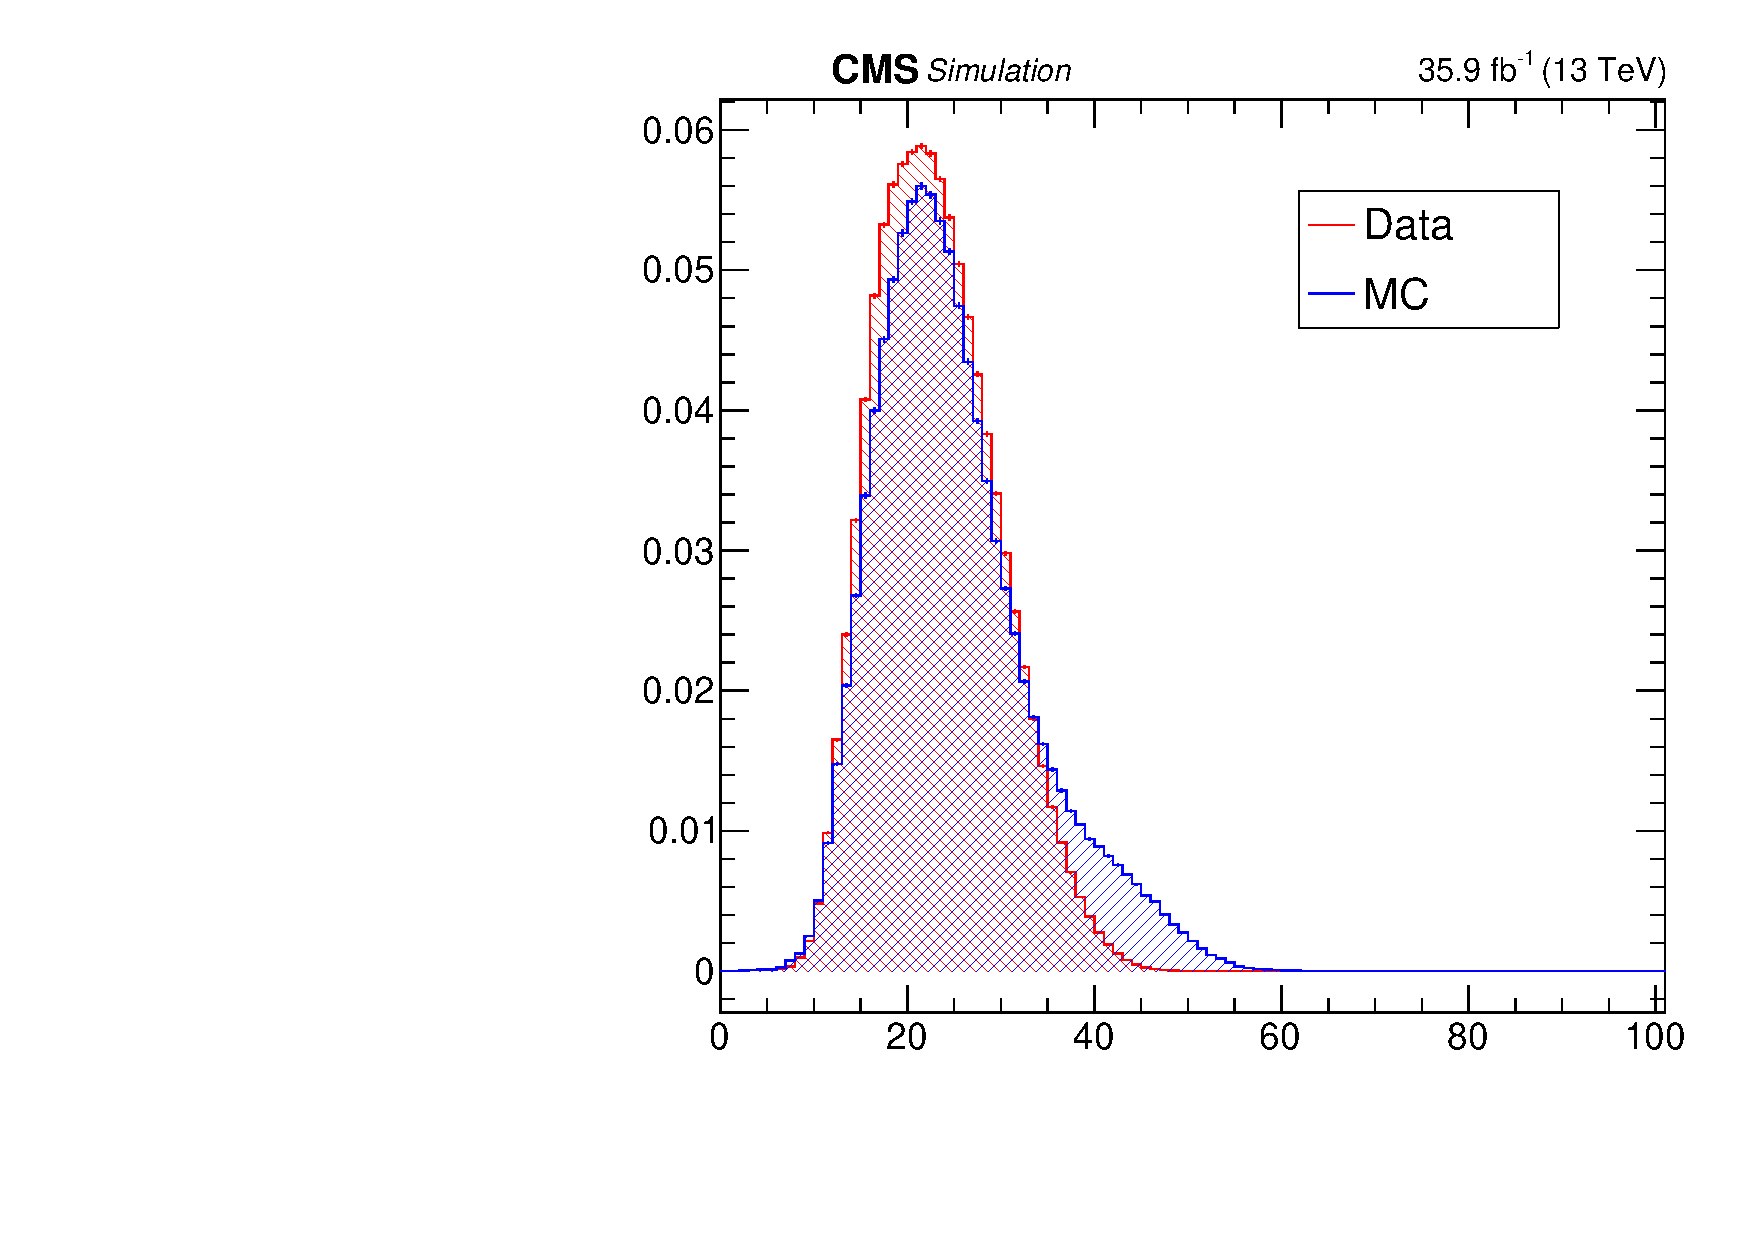
\includegraphics[width=0.8\textwidth]{pileup_2016.pdf}
        \caption{2016}
        \label{fig:pu_2016}
    \end{center}
    \end{subfigure}
    \begin{subfigure}[b]{0.45\textwidth}
    \begin{center}
        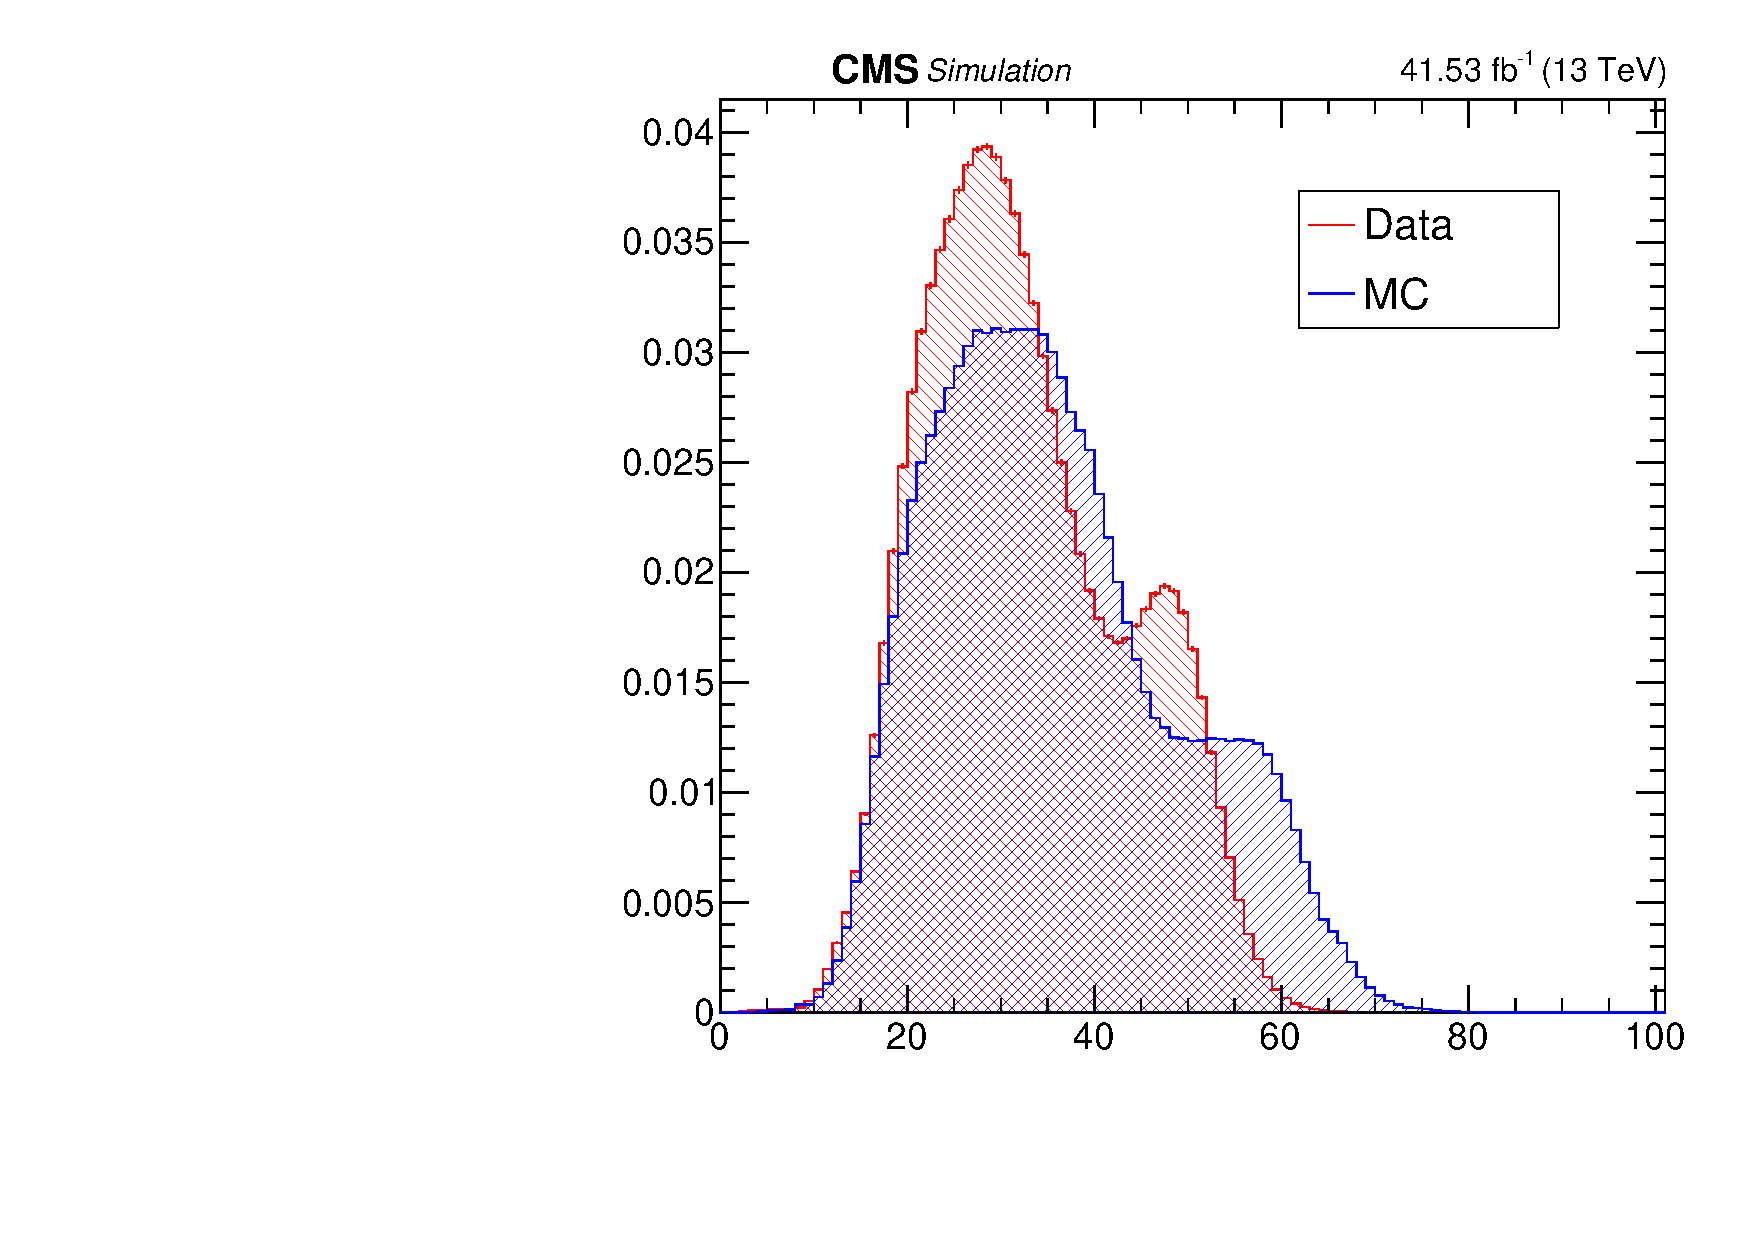
\includegraphics[width=0.8\textwidth]{pileup_2017.pdf}
        \caption{2017}
        \label{fig:pu_2017}
    \end{center}
    \end{subfigure}
    \caption{Nombre d'empilement des données observées et simulées normalisé à 1 pour le processus \ttbar pour l'année (\subref{fig:pu_2016}) 2016 et (\subref{fig:pu_2017}) 2017, ramené à une luminosité de $\mathcal{L} = \SI{1}{\femto \barn^{-1}}$.}
    \label{fig:pu}
\end{center}
\end{figure}
\begin{figure}
\begin{center}
    \begin{subfigure}[b]{0.45\textwidth}
    \begin{center}
        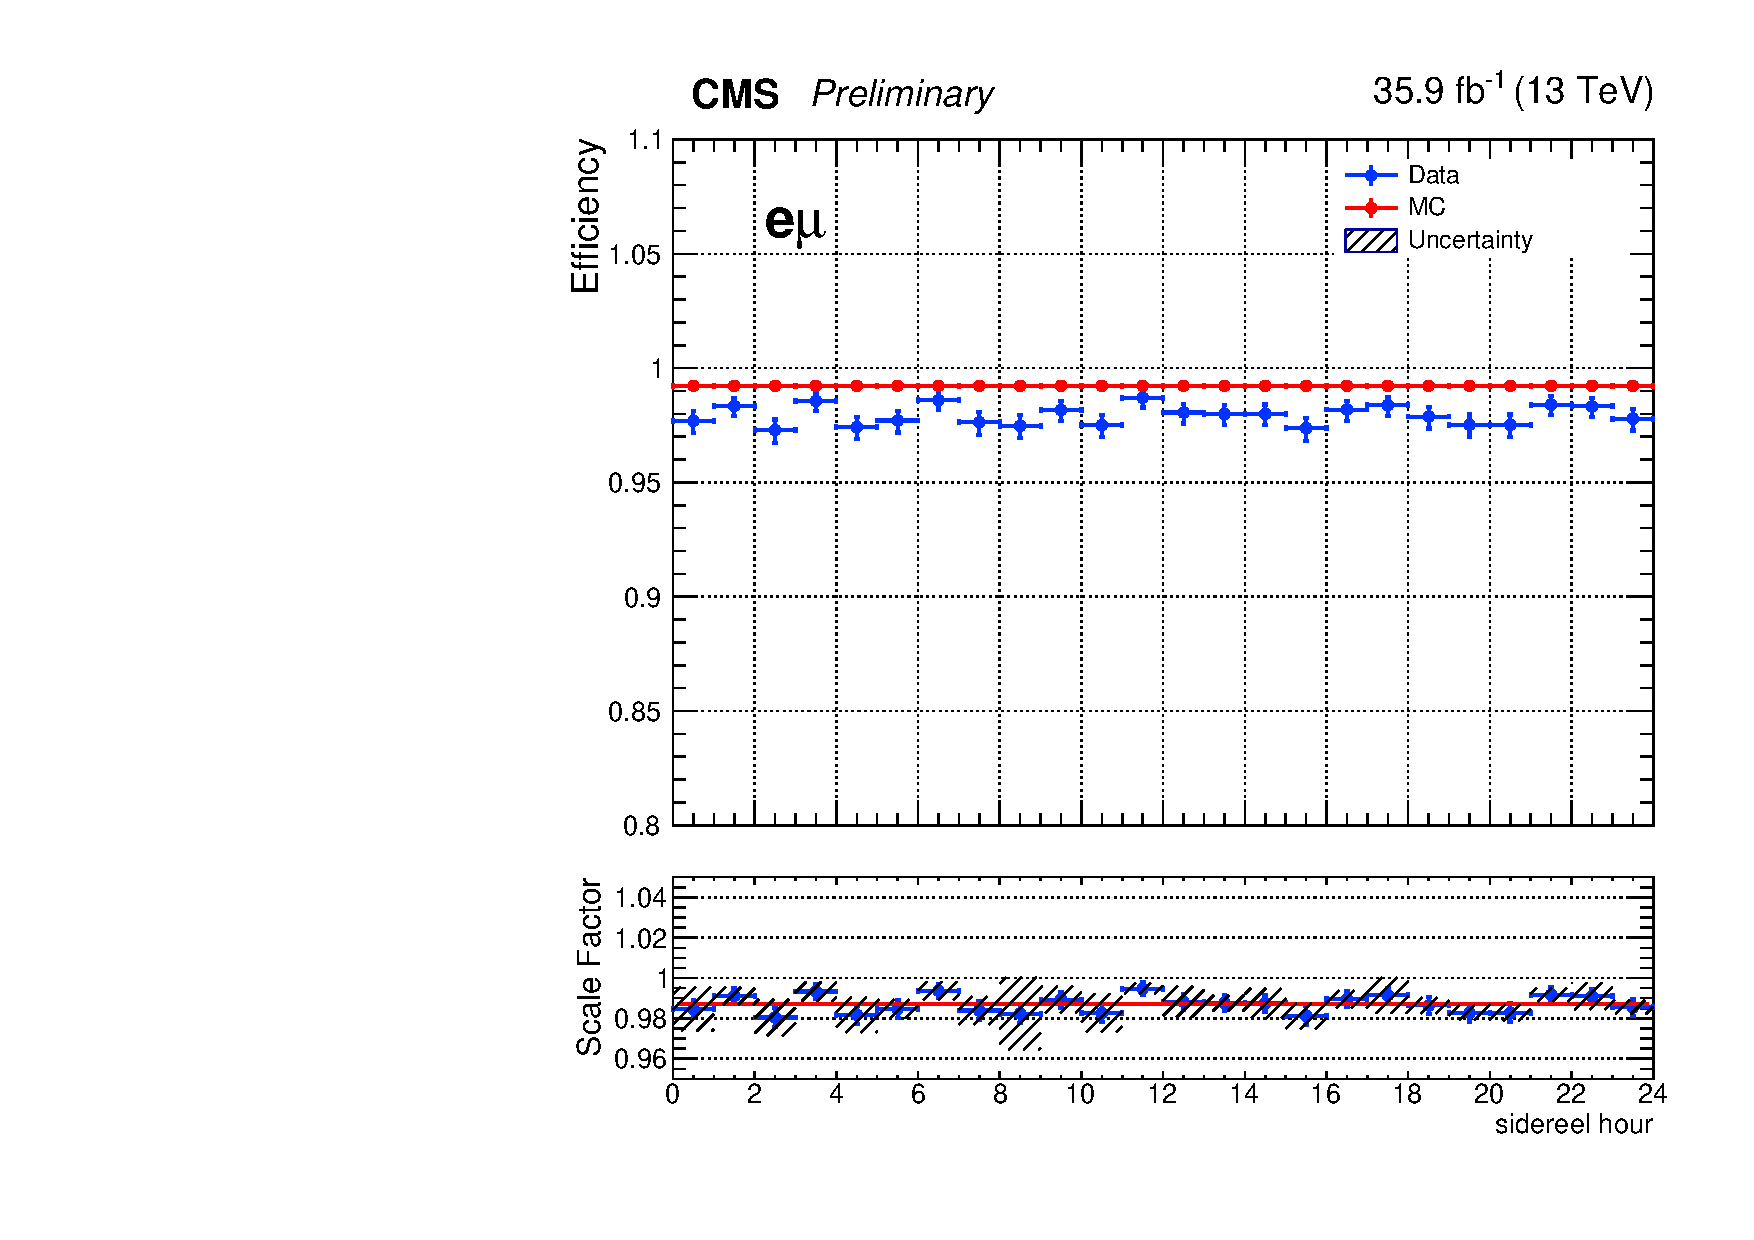
\includegraphics[width=0.9\textwidth]{g_2016_emu_sidereel_FullSystUncBand.pdf}
        \caption{2016}
        \label{fig:emu_2016}
    \end{center}
    \end{subfigure}
    \begin{subfigure}[b]{0.45\textwidth}
    \begin{center}
        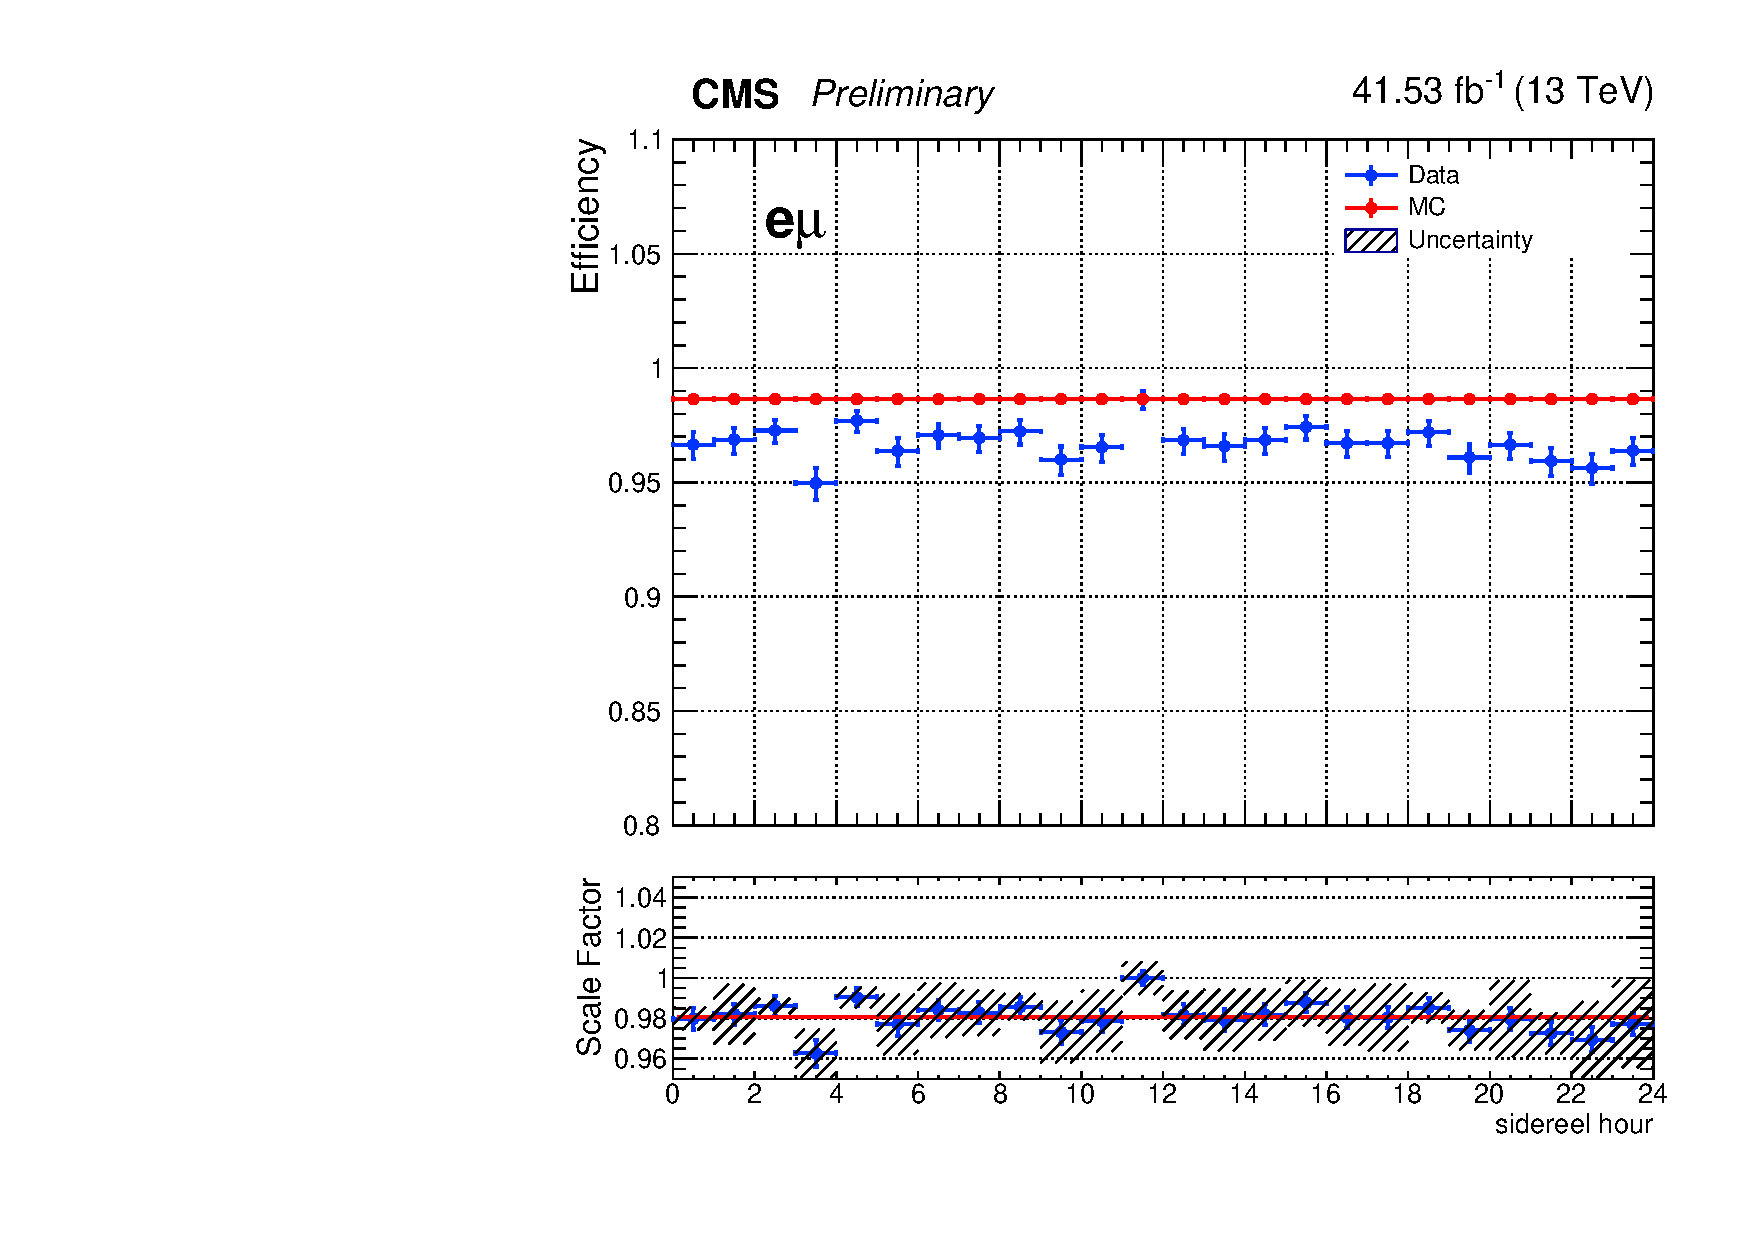
\includegraphics[width=0.9\textwidth]{g_2017_emu_sidereel_FullSystUncBand.pdf}
        \caption{2017}
        \label{fig:emu_2017}
    \end{center}
    \end{subfigure}
    \caption{Comparaison de l'efficacité des chemins de déclenchement  \Pe{}\Pmu fonction du temps sidéral pour l'année (\subref{fig:emu_2016}) 2016 et (\subref{fig:emu_2017}) 2017. Les facteurs correctifs ainsi que leurs incertitudes sont également présentés.}
    \label{fig:emutrig}
\end{center}
\end{figure}


\subsection{Pondérations dues à la reconstruction et identification des leptons}\label{sec:sf}

\begin{description}
\item[Efficacité d'identification et d'isolation des muons et des electrons]
\begin{sloppypar}
Des facteurs correctifs aux efficacités de reconstruction, identification et isolation des leptons sont déterminés. Ces corrections sont appliquées sous formes de poids individuellement pour chaque électron et muon. Ces facteurs dépendent du \pt et $\eta$ de la particule (pour plus de précisions voir \ref{sec:lepton_isolation}). A titre illustratif, les histogrammes des facteurs correctifs pour l'année 2017 de l'identification des électrons et des muons sont présentés respectivement figures  \figurename{\ref{fig:recoelec2017}} et \figurename{\ref{fig:recomuon2017}}. Le reste des facteurs correctifs pour l'isolation des muons et la reconstruction des électrons pour 2016 et 2017 est visible en annexe \ref{app:sfem}.
\end{sloppypar}
\item[Correction de l'efficacité de l'étiquetage $b$]
\begin{sloppypar}
Des facteurs correctifs à l'efficacité de l'étiquetage \Pbottom sont établies en fonction de la saveur du jet au niveau générateur, des propriétés cinématiques du jet et de la valeur de coupure utilisée (voir \ref{btagref}) \cite{Sirunyan_2018}. Le taux de mauvaise identification est aussi corrigé.

La méthode utilisée dans cette analyse est l'utilisation d'un poids $w$ sur les évènements. 
\begin{equation}
 w = \frac{\prod_{i = \textrm{tagged}} \textrm{SF}_i \epsilon_i \quad \prod_{j \neq \textrm{tagged}} (1-\textrm{SF}_j \epsilon_j)  }{\prod_{i = \textrm{tagged}} \epsilon_i \quad \prod_{j \neq \textrm{tagged}} (1-\epsilon_j) }
\end{equation}
où $\textrm{SF}_i$ est le facteur correctif du jet $i$ et $\epsilon_i$ l'efficacité de l'étiquetage \Pbottom évaluée sur l'ensemble des échantillons Monte-Carlo de l'analyse. A titre illustratif, un histogramme des facteurs correctifs pour l'année 2017 avec l'algorithme DeepCSV est présenté à la figure \figurename{\ref{fig:deepcsv2017}}. Le reste des facteurs correctifs pour l'étiquetage \Pcharm et l'étiquetage des jets légers pour 2016 et 2017 est visible en annexe \ref{app:sfb}.
\end{sloppypar}
\item[Correction de l'impulsion transverse du quark top]
\begin{sloppypar}
Plusieurs analyses \ttbar, au LHC, ont montré que la distribution du \pt du quark \Ptop  est déplacée en moyenne vers de plus basses valeurs dans les données que dans les simulations. Dans cette analyse une correction proposée par la collaboration est effectuée. Il s'agit d'appliquer un poids aux évènements en fonction du \pt du quark \Ptop et en fonction du type de simulation utilisé. Dans notre cas, l'utilisation de simulations générées avec \texttt{POWHEG} et \texttt{Pythia8\,} implique une correction de type :
\begin{equation}
\textrm{SF}(\pt) = e^{0.0615-0.0005\pt}
\end{equation}
où \textrm{SF} est le facteur correctif.
La déduction de la valeur du facteur correctif est faite à partir du graphe présenté dans la figure \figurename{\ref{fig:toprew}}. 
La correction est dédiée uniquement aux échantillons de simulations \ttbar et se fait par l'application du poids $w$ défini par :
\begin{equation}
w = \sqrt{\textrm{SF}(\pt{}_1)^2 + \textrm{SF}(\pt{}_2)^2}
\end{equation}
où les indices $1$ et $2$ représentent les deux quarks \Ptop impliqués dans les évènements.
\end{sloppypar}
\end{description}

\begin{figure}
    \begin{center}
        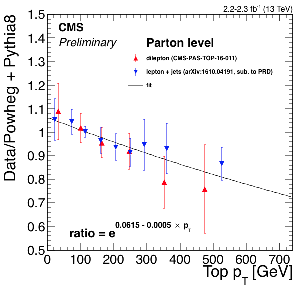
\includegraphics[width=0.5\textwidth]{TopPt_DATA_PWHGP8.pdf}
        \caption{Histogramme présentant l'écart en \pt dans les échantillons avec quark \Ptop avec la mesure dans les données.}
        \label{fig:toprew}
    \end{center}
\end{figure}

\begin{figure}
    \begin{center}
        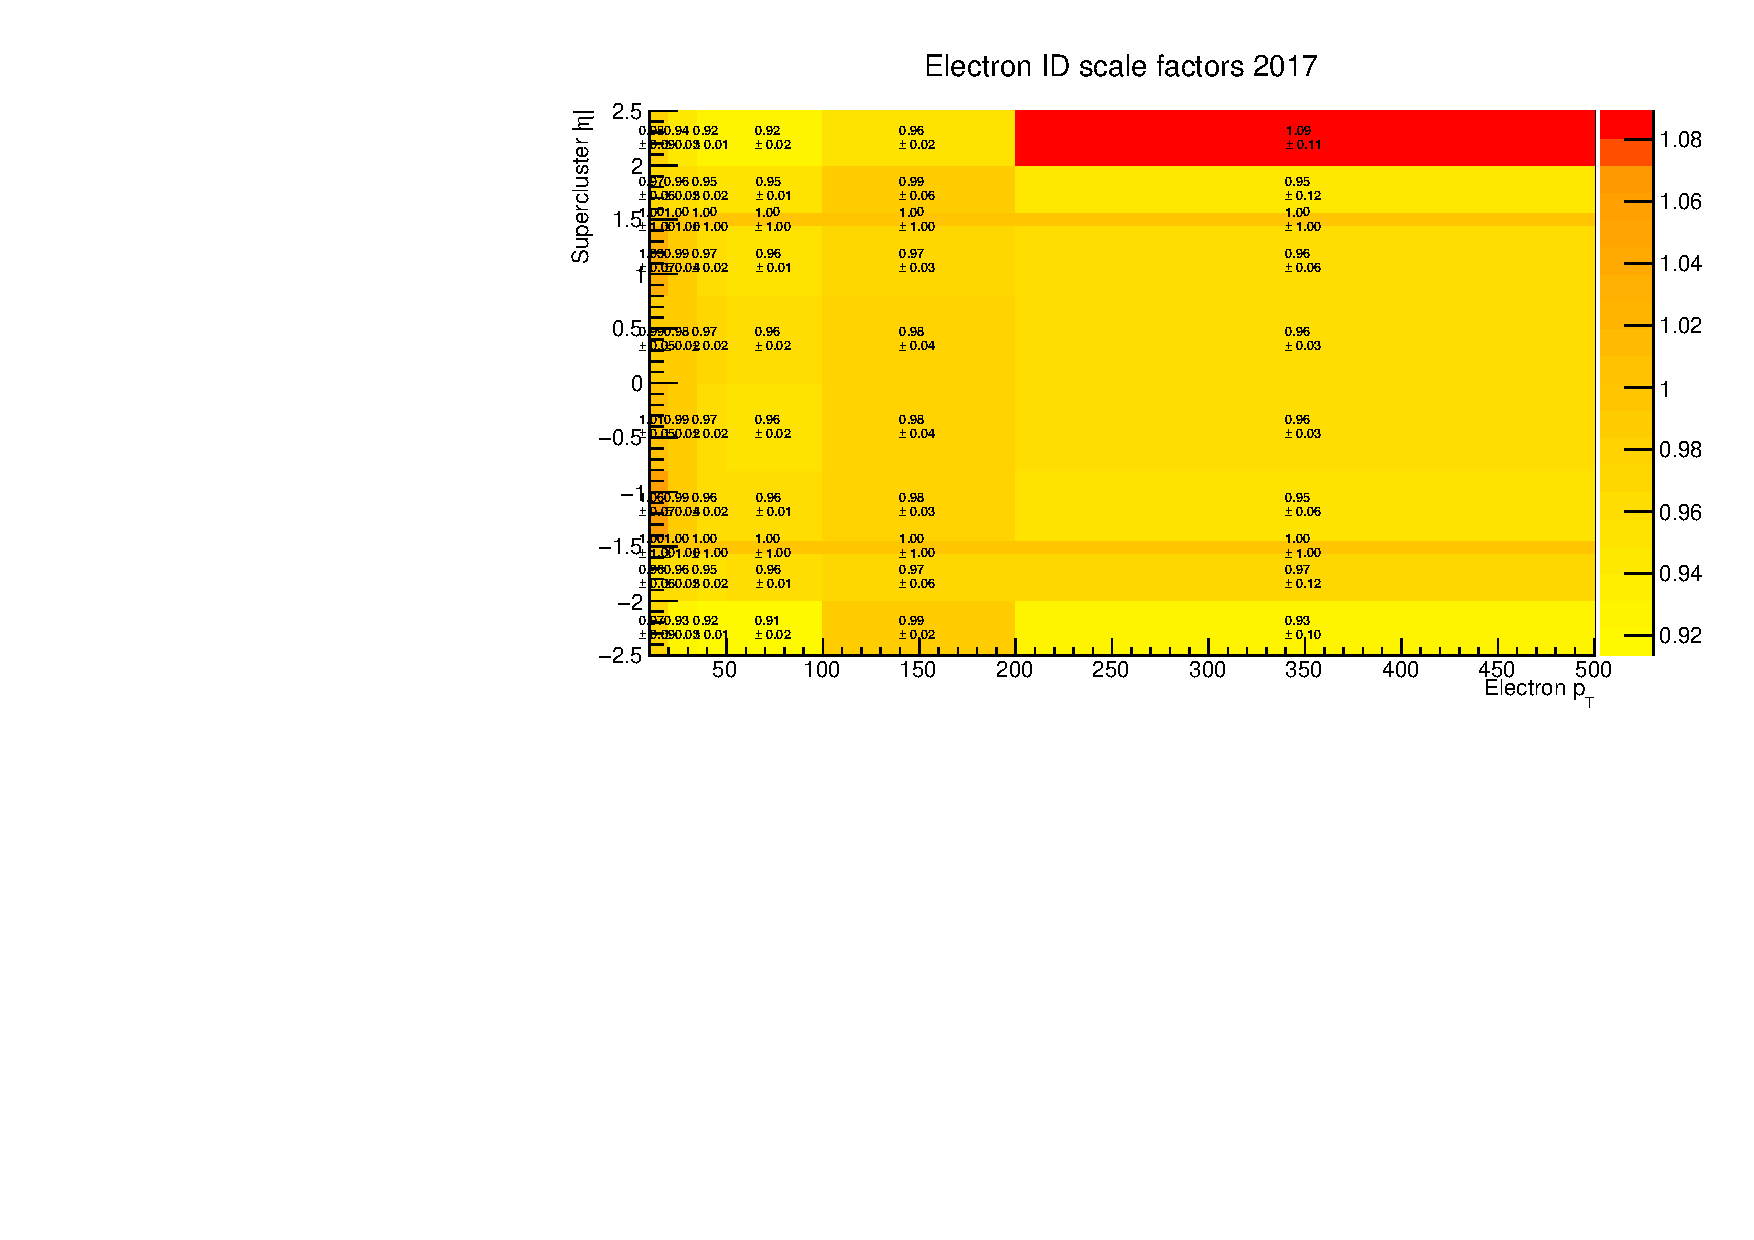
\includegraphics[width=0.5\textwidth]{Canvas_Electron_SF_2017_ID.pdf}
        \caption{Histogramme 2D des facteurs correctifs d'identification des électrons pour l'année 2017. L'abscisse est l'impulsion transverse \pt du jet considéré et l'ordonnée est sa pseudo-rapidité en valeur absolue $|\eta|$.}
        \label{fig:recoelec2017}
    \end{center}
\end{figure}

\begin{figure}
    \begin{center}
        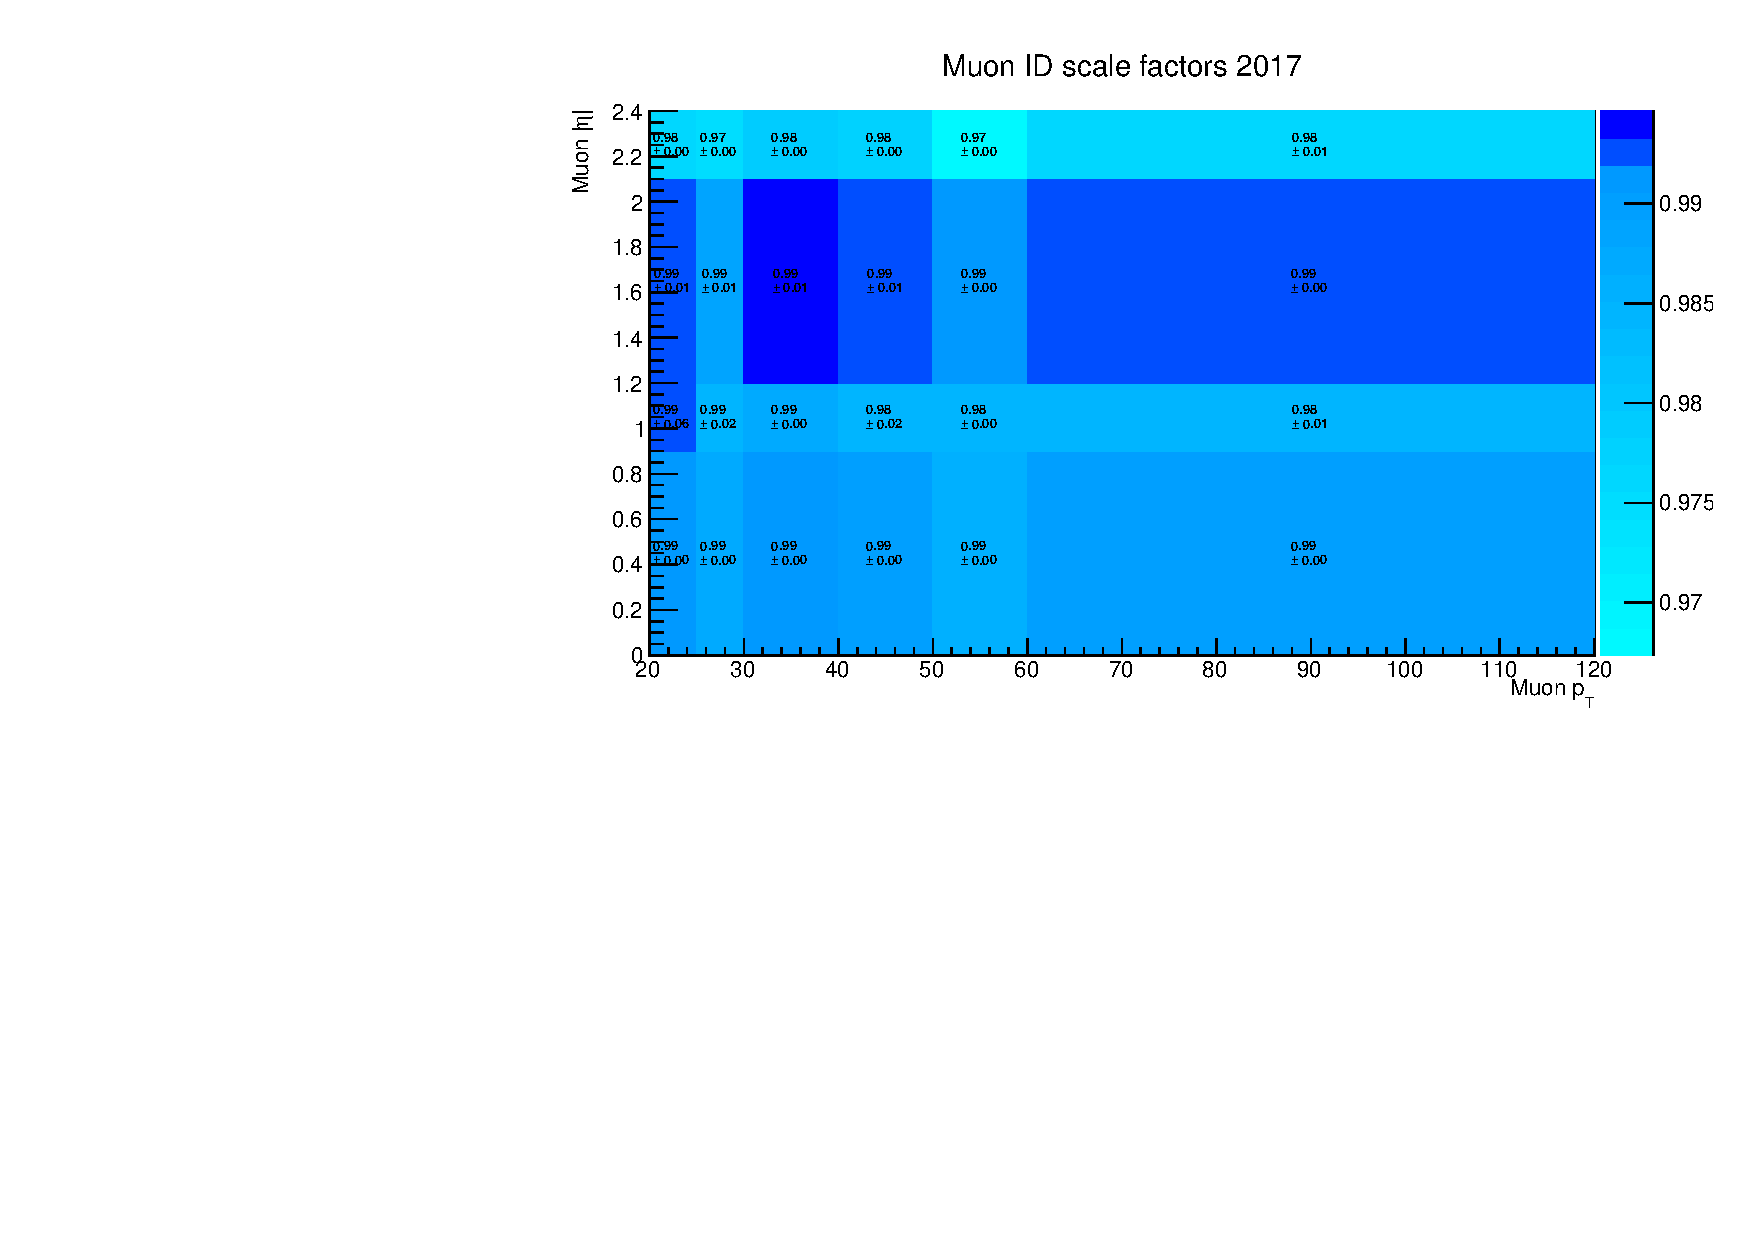
\includegraphics[width=0.5\textwidth]{Canvas_Muon_SF_2017_ID.pdf}
        \caption{Histogramme 2D des facteurs correctifs d'identification des muons pour l'année 2017. L'abscisse est l'impulsion transverse \pt du jet considéré et l'ordonnée est sa pseudo-rapidité en valeur absolue $|\eta|$.}
        \label{fig:recomuon2017}
    \end{center}
\end{figure}



\begin{figure}
    \begin{center}
        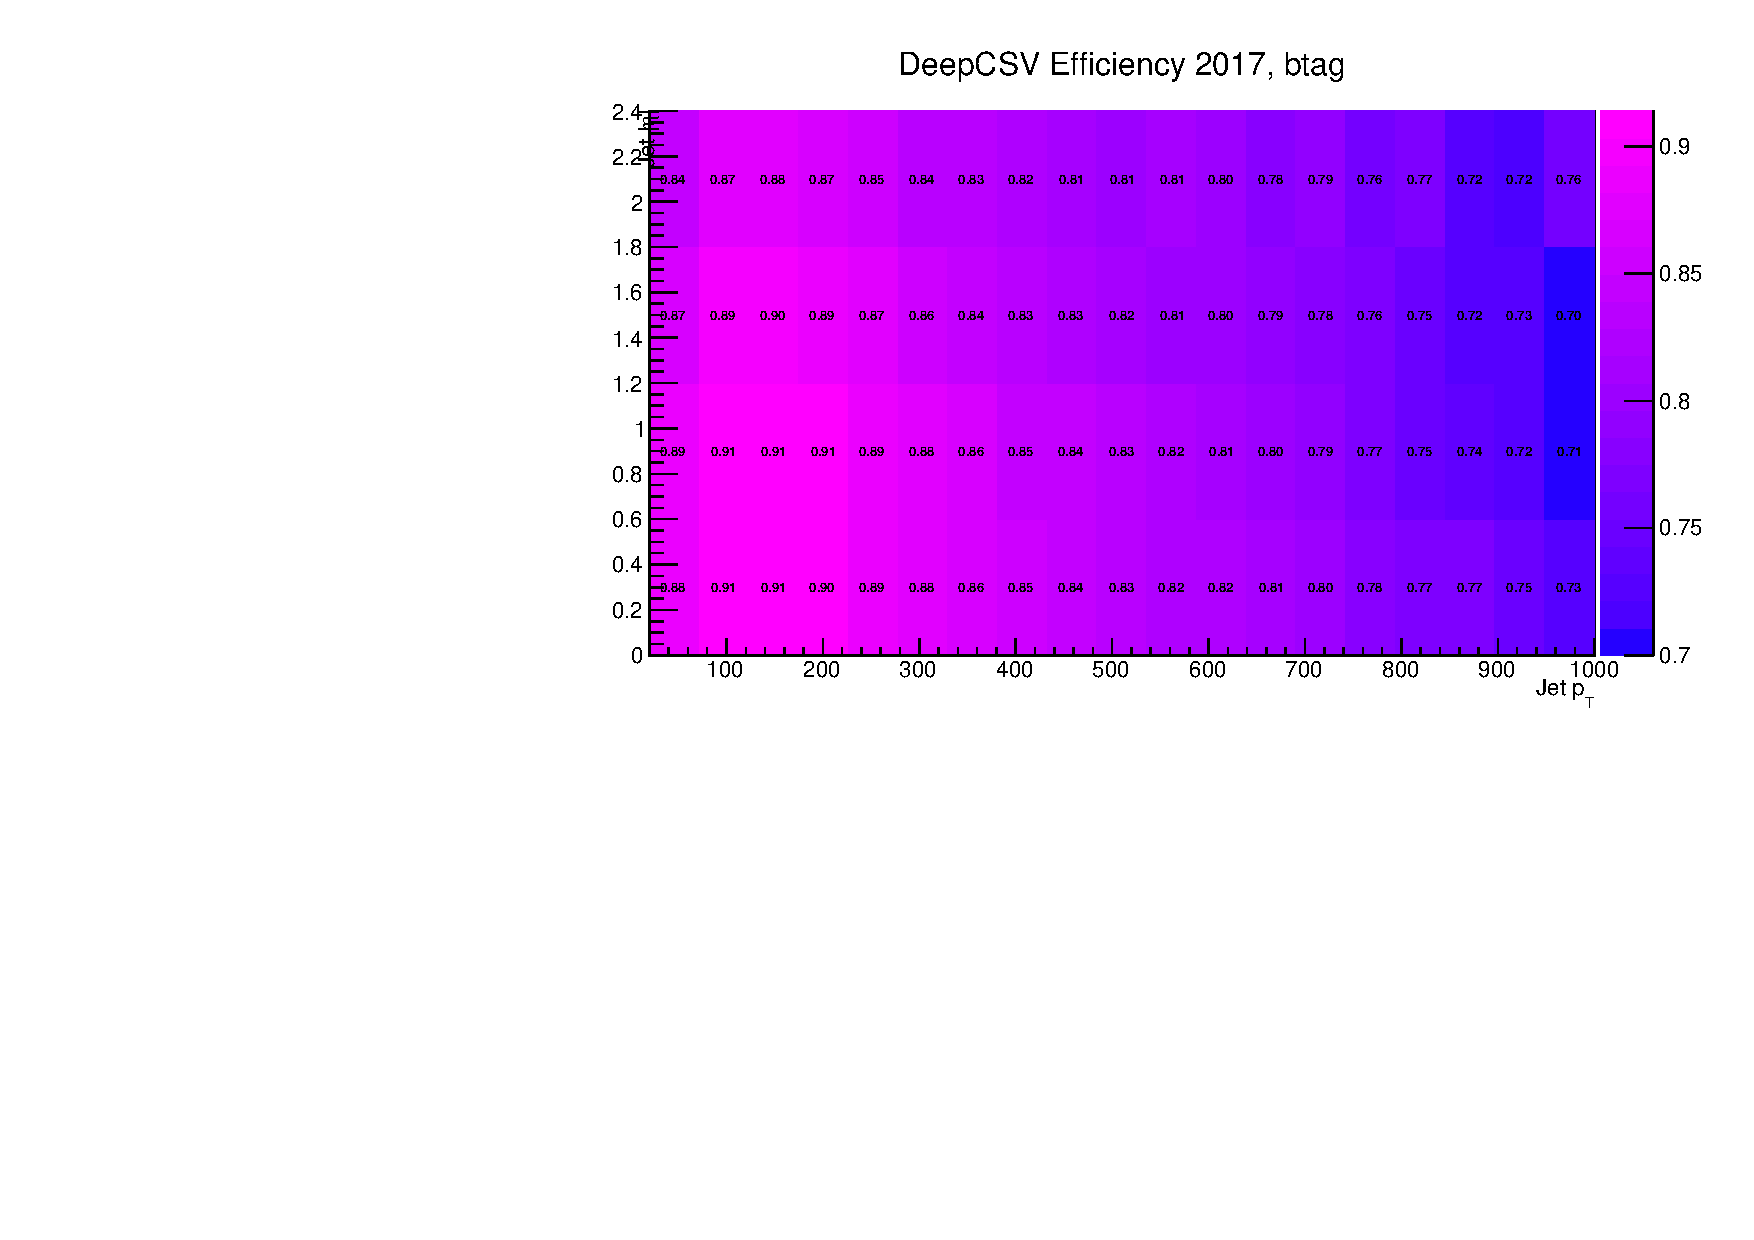
\includegraphics[width=0.5\textwidth]{Canvas_DeepCSV_SF_2017_btag.pdf}
        \caption{Histogramme 2D de l'efficacité de l'étiquetage \Pbottom{} avec l'algorithme DeepCSV pour l'année 2017. L'abscisse est l'impulsion transverse \pt du jet considéré et l'ordonnée est sa pseudo-rapidité en valeur absolue $|\eta|$.}
        \label{fig:deepcsv2017}
    \end{center}
\end{figure}


\section{Comparaison données/simulations}
\begin{sloppypar}
Pour valider la chaîne d'analyse, il est de rigueur d'utiliser des observables de contrôle. Il s'agit d'observables qui ne prennent pas explicitement en compte le paramètre caractéristique de notre analyse qu'est le temps sidéral. 
\end{sloppypar}
\subsection{Validation des coupures}

Pour valider la sélection, on procède à un décompte du nombre d'évènements de chaque échantillon après chaque coupure. Ces décomptes sont présentés sous forme de tableaux appelés \emph{cut-flow} pour l'année 2016 (\tablename{\ref{tab:cutflow2016}}) et pour l'année 2017 (\tablename{\ref{tab:cutflow2017}}).
On peut visualiser l'efficacité de sélection avec une proportion d'évènements \ttbar de \SI{\sim 67}{\%} après la sélection d'évènements comportant exactement deux leptons contre une proportion de \SI{\sim 93}{\%} après la sélection d'évènements comportant exactement deux leptons, au moins deux jets dont au moins un étiqueté \Pbottom.

On voit une différence du nombre d'évènements entre les données et les simulations d'environ \SI{10}{\%} pour 2016 et \SI{5}{\%} pour 2017. Ce déficit observé dans les données est compatible avec ce qui a été observe dans d'autres analyses \ttbar de CMS.

\begin{figure}[h]
    \begin{center}
    \begin{tabular}{c|rl@{\hspace{3em}}rl@{\hspace{3em}}rl}
    \noalign{\smallskip}\hline\noalign{\smallskip}
     & \multicolumn{2}{c}{2 leptons} & \multicolumn{2}{c}{2 jets} & \multicolumn{2}{c}{1 b-jet} \\ 
    \noalign{\smallskip}
    \hline \hline
    \noalign{\smallskip}
    $t\bar{t}$ signal & 231974 &[66.8\%] & 182037 &[90.5\%] & 172242 &[93.5\%]\\ 
    \noalign{\smallskip}\hline\noalign{\smallskip}
    TTX               &  1389  &[0.4\%] & 1609   &[0.8\%]  & 537    &[0.3\%]   \\ 
    single top        &  21183 &[6.1\%] &  9253  &[4.6\%]  & 8711   &[4.7\%]   \\ 
    dibosons          &  24656 &[7.1\%] &  2011  &[1.0\%]    & 732    &[0.4\%]   \\ 
    V$+$Jets          &  68064  &[19.6\%] &  6235   &[3.1\%]  & 2110   &[1.1\%]   \\ 

        \noalign{\smallskip}\hline\noalign{\smallskip}
    total MC          & 347266 &[100\%]  &   201145 &[100\%]  & 184331 &[100\%]\\ 
    total data &  &                       &                & &166037& \\ 
        \noalign{\smallskip}\hline\noalign{\smallskip}
    \end{tabular}

    \end{center}
    \caption{Nombres d'évènements de tous les échantillons après chaque coupure pour l'année 2016.}
    \label{tab:cutflow2016}
\end{figure}

\begin{figure}[h]
    \begin{center}
    \begin{tabular}{c|rl@{\hspace{3em}}rl@{\hspace{3em}}rl}
    \noalign{\smallskip}\hline\noalign{\smallskip}
     & \multicolumn{2}{c}{2 leptons} & \multicolumn{2}{c}{2 jets} & \multicolumn{2}{c}{1 b-jet} \\ 
    \noalign{\smallskip}    
    \hline \hline
    \noalign{\smallskip}
    $t\bar{t}$ signal & 258747 &[67.9\%] & 207186 &[90.6\%] & 195837 &[93.6\%]\\ 
    \noalign{\smallskip}\hline\noalign{\smallskip}
    TTX               & 857    &[0.2\%] & 686    &[0.3\%]  & 642    &[0.3\%]   \\ 
    single top        & 24808  &[6.5\%] & 11372   &[4.9\%]  & 10068  &[4.8\%]   \\ 
    dibosons          & 27698  &[7.3\%] & 2297   &[1.0\%]    & 665    &[0.3\%]   \\ 
    V$+$Jets          & 69124  &[18.1\%] & 7206    &[3.2\%]  & 2167   &[1.0\%]   \\ 

        \noalign{\smallskip}\hline\noalign{\smallskip}
    total MC          & 381234 &[100\%]  & 228746 &[100\%]  & 209379 &[100\%]\\ 
    total data &  &                      &              &   & 199897& \\ 
        \noalign{\smallskip}\hline\noalign{\smallskip}
    \end{tabular}
    \end{center}
    \caption{Nombres d'évènements de tous les échantillons après chaque coupure pour l'année 2017.}
    \label{tab:cutflow2017}
\end{figure}


\subsection{Comparaison sur des observables}

Dans le but de vérification de la chaîne d'analyse on peut également faire un tracé de la comparaison données/simulations pour différentes observables. Il est à noter que ces comparaisons ne doivent pas intégrer l'élément central de notre analyse qu'est le temps. En effet, ces comparaisons doivent servir de vérifications. Or, comme il le sera précisé dans la section \ref{sec:final}, dans le but d'assurer une expérience en aveugle, les éléments caractéristiques de notre analyse doivent être évités lors des phases de tests.

La figure \figurename{\ref{fig:comp_mdilep}} présente les comparaisons données/simulations de la masse dilepton pour l'année 2016 et 2017. Ces comparaisons sont dites \emph{pre-fits} elle ne comporte donc que les incertitudes statistiques. Les incertitudes systématiques seront présentées puis évaluées dans la suite de ce chapitre.

\begin{figure}
    \begin{subfigure}[b]{0.5\textwidth}
    \begin{center}
        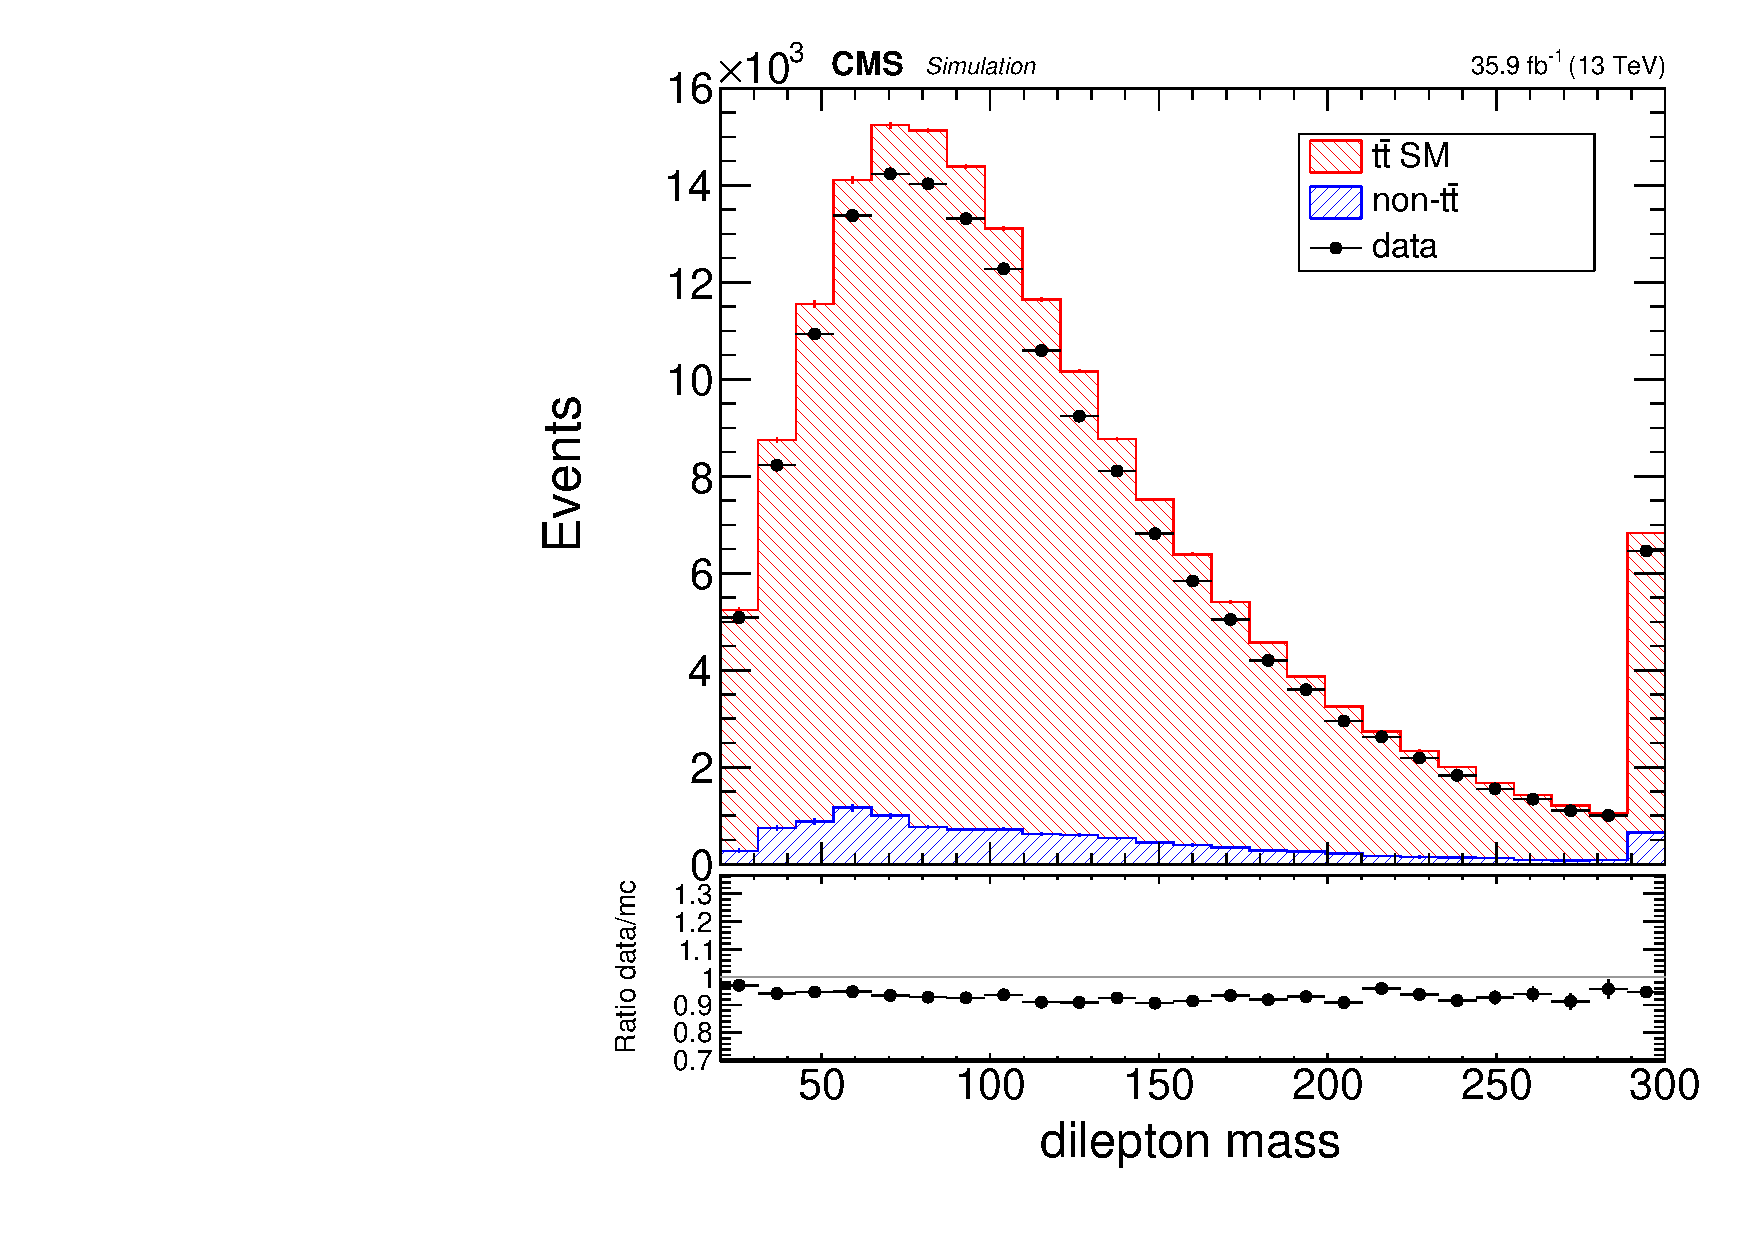
\includegraphics[width=0.8\textwidth]{m_dilep_2016.pdf}
        \caption{2016}
        \label{fig:mdilep_2016}
    \end{center}
    \end{subfigure}
    \begin{subfigure}[b]{0.5\textwidth}
    \begin{center}
        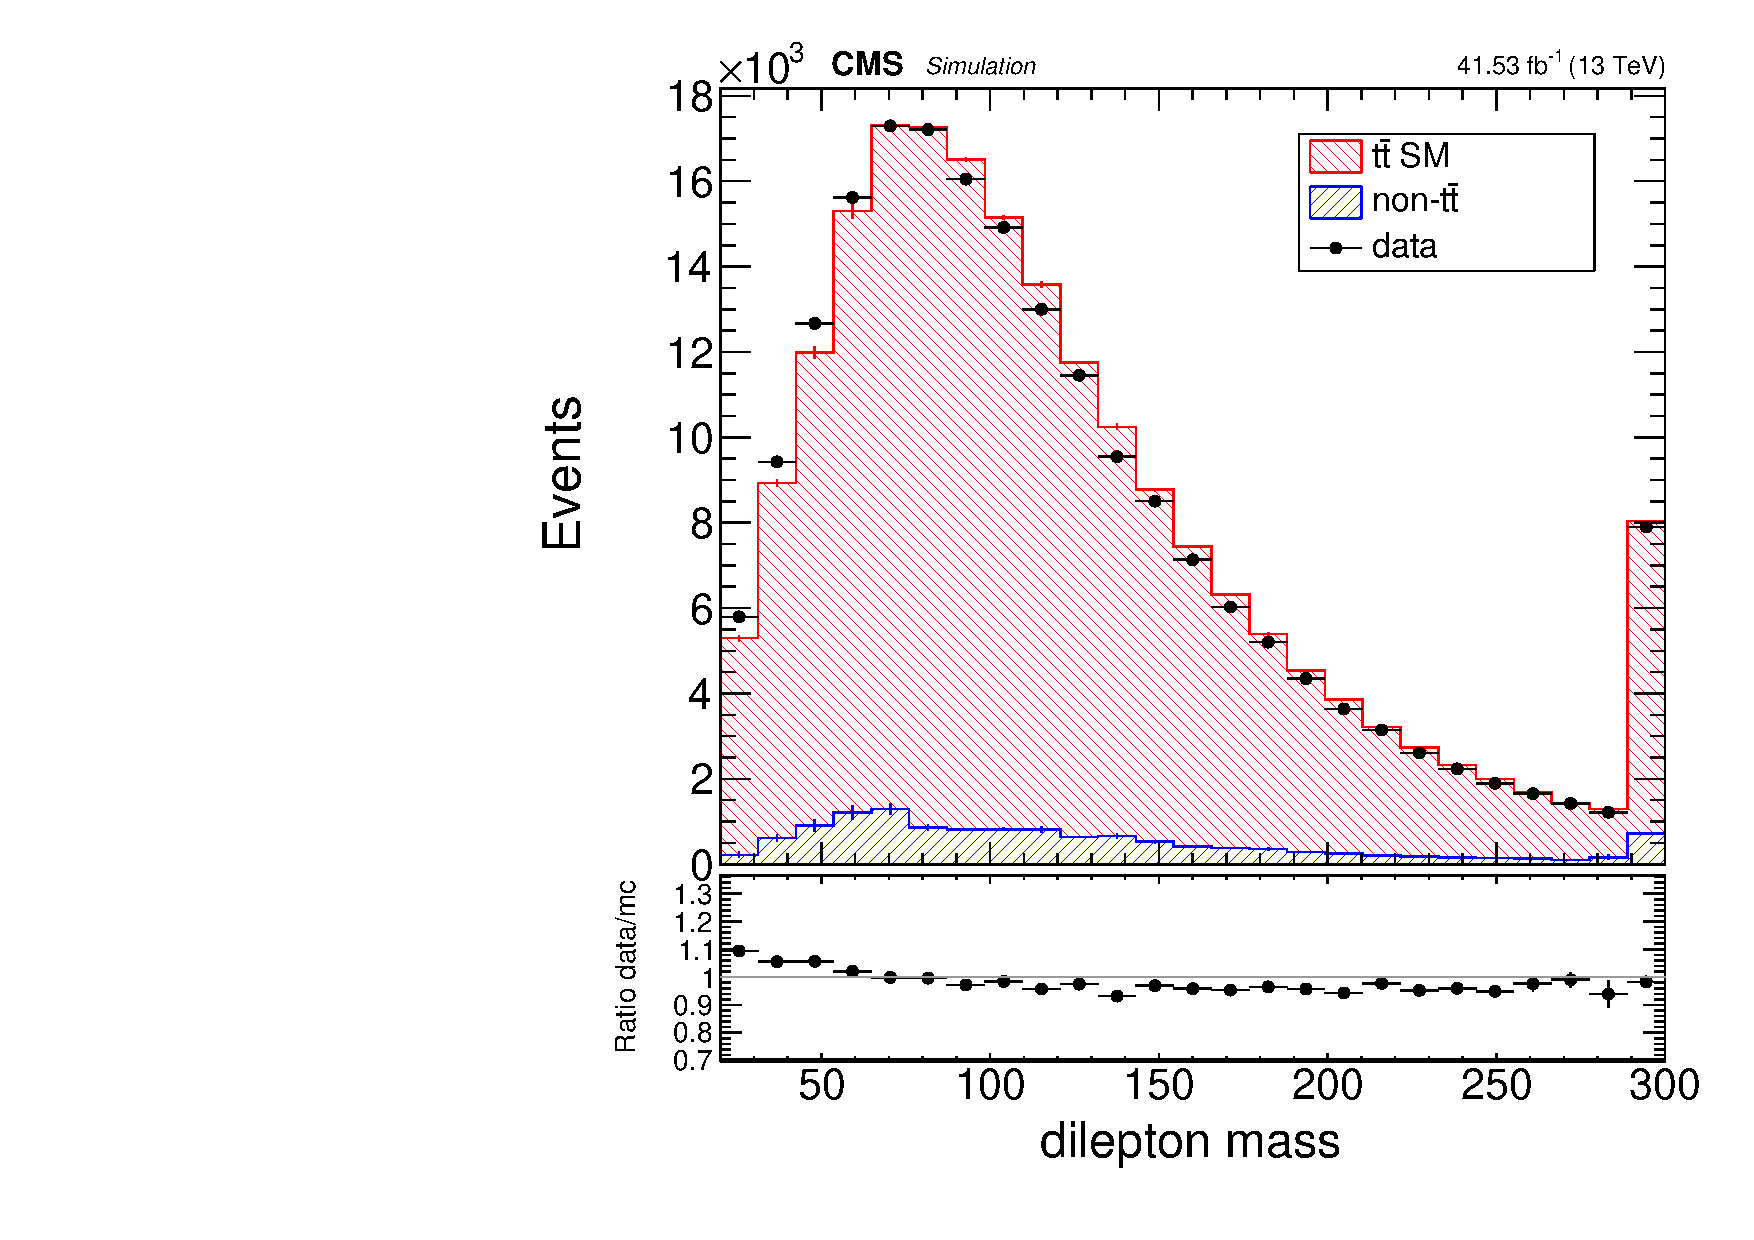
\includegraphics[width=0.8\textwidth]{m_dilep_2017.pdf}
        \caption{2017}
        \label{fig:mdilep_2017}
    \end{center}
    \end{subfigure}
    \caption{Comparaison données/Monte-Carlo pour la masse dilepton pour l'année (\subref{fig:mdilep_2016}) 2016 et (\subref{fig:mdilep_2017}) 2017.}
    \label{fig:comp_mdilep}
\end{figure}

Un ensemble de comparaisons données/simulations sur d'autres observables est présenté dans l'annexe \ref{comparaison}.


\section{Test statistique et incertitudes systématiques}

L'étape finale de l'analyse consiste à déterminer la présence d'un signal ou non en fonction des observations. Autrement dit, évaluer la valeur des coefficients  $c_{\mu\nu}$ ainsi que l'ensemble de leurs incertitudes. Pour cela, on va utiliser un estimateur statistique appelé maximum de vraisemblance (\emph{maximum likelihood estimation}).

\subsection{L'ajustement par maximum de vraisemblance}\label{sec:likelihood}

Pour extraire le nombre total d'évènements de signal $N_s$, le test statistique consiste en une maximisation d'une fonction de vraisemblance $\mathfrak{L}$ définie comme produit des probabilités de Poisson $\mathfrak{P}(n_i \vert \rho_i(\mu,\vec{\vartheta}))$ d'observer $n_i$ évènements dans chaque bin $i$ de l'histogramme de la variable discriminante : 

\begin{equation}
    \mathfrak{L}(N_s, \vec{\vartheta}) = \prod_{i=0}^{N_\mathrm{bin}} \mathfrak{P}(n_i, \rho_i(\mu,\vec{\vartheta})) 
\end{equation}
avec la distribution de Poisson :
\begin{equation}
\mathfrak{P}(n_i \vert \rho_i(\mu,\vec{\vartheta})) = \frac{\rho_i e^{-\rho_i}}{n_i!}
\end{equation}
Cette distribution de Poisson est pilotée par la fonction de densité de probabilité $\rho_i(\mu,\vec{\vartheta})$ définie par : 
\begin{equation}\label{Poisson}
\rho_i(\mu,\vec{\vartheta}) = \mu s_i(\vec{\vartheta}) + b_i(\vec{\vartheta})
\end{equation}
avec, pour chaque bin $i$, $s_i$ le nombre d'évènements de signal et $b_i$ le nombre d'évènement de bruit de fond. Chacun de ces nombres d'évènements est fonction d'un ensemble de paramètres contraints par des PDF : $\vec{\vartheta}$ nommés paramètres de nuisance (\emph{nuisance parameter}) correspondant aux sources d'incertitudes présentées dans la section \ref{sec:incertitudes}. La variation de ces paramètres peut induire une variation des nombres $s_i$ et $b_i$. La dernière variable $\mu$ est le modificateur d'intensité du signal (\emph{signal strength modifier}) fonction des nombres d'évènements observés et prédits et défini par :
\begin{equation}
\mu = \frac{N_\mathrm{observé}}{N_\mathrm{predit}}
\end{equation}
C'est cette variable qui sert à l'ajustement du maximum de vraisemblance. 

Dans notre cas, le modificateur $\mu$ est proportionnel aux coefficients $c_{\mu\nu}$. 
Ceci s'explique par le fait que les coefficients $c_{\mu\nu}$ est un facteur multiplicatif du nombre d'évènements de \ttbar additionnels par rapport au Modèle Standard. De plus, les  termes quadratiques en $c_{\mu\nu}$ sont négligés; on ne considère que les termes linéaires entre le Modèle Standard et le SME. Ainsi, l'ajustement nous donnera directement l'estimation de la valeur des $c_{\mu\nu}$ ainsi que leurs incertitudes. 
\newline

Pour l'évaluation des paramètres de nuisances, trois types d'incertitudes peuvent être décrites \cite{CMSAtlasStat} :
\begin{description}
\item[Incertitudes de normalisation] 
\begin{sloppypar}
Ces incertitudes regroupent les contraintes de type facteurs multiplicatifs  $\mathfrak{C}_\textrm{facteurs}(\vartheta,\tilde{\vartheta})$ appliqués sur le nombre d'évènements de signal ou de bruit de fond mais également les contraintes sur les incertitudes d'origine statistique $\mathfrak{C}_\textrm{statistique}(\vartheta,\tilde{\vartheta})$ . Chacune de ces contraintes représente la probabilité que ce paramètre
prenne la valeur $\vartheta$, sachant que la meilleure estimation de ce dernier est $\tilde{\vartheta}$, obtenue par des mesures annexes.

Dans le premier cas, ces contraintes sont évaluées par des fonctions de densités de probabilités log-normales :
\begin{equation}
\mathfrak{C}_\textrm{facteurs}(\vartheta,\tilde{\vartheta}) = \frac{1}{\sqrt{2\pi} \ln(1+x)}\frac{1}{\vartheta}\exp\left( - \frac{\ln^2(\vartheta/\tilde{\vartheta})}{2 \ln^2(1+x)} \right)
\end{equation}
où $x$ est l'incertitude relative sur l'observable contrainte et $\tilde{\vartheta}$ est la meilleure estimation du paramètre de nuisance $\vartheta$. La fonction log-normale a l'avantage de tendre vers 0 quand $\vartheta$ tend vers 0, contrairement à une gaussienne.

Dans le second cas, les incertitudes d'origine statistique sont évaluées par 
\begin{equation}
\mathfrak{C}_\textrm{statistique}(\vartheta,\tilde{\vartheta}) = \frac{1}{\kappa\Gamma(\tilde{\vartheta}+1)}\left(\frac{\vartheta}{\kappa}\right)^{\tilde{\vartheta}} \exp\left(-\frac{\vartheta}{\kappa}\right)
\end{equation}
où $\Gamma$ est la fonction gamma d'Euler et $\kappa$ le rapport attendu entre $\vartheta$ et $\tilde{\vartheta}$. La valeur de $\kappa$ possède sa propre incertitude traitée comme une contrainte log-normale supplémentaire.
\end{sloppypar}
\item[Incertitudes de forme] 
\begin{sloppypar}
Ces incertitudes systématiques sont basées sur un traitement des distributions des variables discriminantes avec un  "morphing vertical" \cite{Conway}. Pour chaque source d'incertitude, une distribution centrale (ou nominale) $h_0$ ainsi que des distributions normalisées à $\pm 1 \sigma$ de l'incertitude $h^\pm$ sont produites. Pour traiter ces distributions par interpolation, un paramètre $\lambda$ est ajouté au modèle de vraisemblance et les effets de plusieurs incertitudes de forme sont additifs.

Lors de la maximisation de la fonction $\mathfrak{L}$, est réalisée l'interpolation :
\begin{equation}
    h(\vec{\lambda}) = h_0 + \sum_{j}\left( a(\lambda_j) h^{+}_{j} +  b(\lambda_j) h^{0}_{j} +  c(\lambda_j) h^{-}_{j} \right)
\end{equation}
avec
\footnotesize{
\begin{equation*} 
a = \left\lbrace \begin{matrix}
\lambda(\lambda + 1)/2 &\textrm{pour } |\lambda| \leq 1 \\ 0 &\textrm{pour } \lambda < -1 \\ \lambda &\textrm{pour } \lambda > 1
\end{matrix} \right. \quad 
b = \left\lbrace \begin{matrix}
-\lambda^2 &\textrm{pour } |\lambda| \leq 1 \\ -|\lambda| &\textrm{pour } |\lambda| > 1
\end{matrix} \right. \quad
c = \left\lbrace \begin{matrix}
\lambda(\lambda - 1)/2 &\textrm{pour } |\lambda| \leq 1 \\ |\lambda| &\textrm{pour } \lambda < -1 \\ 0 &\textrm{pour } \lambda > 1
\end{matrix} \right. 
\end{equation*}
}
\end{sloppypar}
\item[Incertitudes statistiques sur le Monte-Carlo] 
\begin{sloppypar}
Ces incertitudes statistiques sont gérées par la méthode Barlow-Beeston \cite{Barlow}. L'idée consiste en la création d'une pseudo-incertitude de forme en évaluant la variation de la quantité d'évènements dans chaque bin de la distribution de la variable discriminante. L'incertitude totale $e_\mathrm{tot}$ sur l'ensemble des processus $p$ est déterminée par :
\begin{equation}
e^2_\mathrm{tot} = \sum_{i\in p}^{N_\mathrm{bin}} e^2_i.
\end{equation}
où $i \in p$ représente l'ensemble des bins $i$ des différents processus. Dans  notre analyse, on utilisera une méthode Barlow-Beeston dite \emph{light}, pour laquelle l'incertitude statistique du     Monte-Carlo est évaluée uniquement sur la sommes des évènements des différents processus (et non pour chaque processus individuel).
\end{sloppypar}
\end{description}

\subsection{La méthode $\textrm{CL}_s$}

L'enjeu est maintenant d'estimer la meilleure concordance entre les résultats de l'analyse et l'hypothèse de bruit de fond uniquement ou l'hypothèse signal plus bruit de fond. En vertu du lemme de Neyman-Pearson \cite{Neyman}, la meilleure concordance est obtenue par le test statistique de profil du rapport de vraisemblance (\emph{profile likelihood ratio}) :
\begin{equation}
    q_\mu = -2 \ln\left( \frac{\mathfrak{L}(\textrm{données} | \mu, \hat{\vec{\vartheta}}_\mu)) }{\mathfrak{L}(\textrm{données} | \hat{\mu}, \hat{\vec{\vartheta}}_\mu) }  \right) \quad\textrm{avec}\quad 0 \leq \hat{\mu} \leq \mu
\end{equation}
avec "données" qui réfère aux quantités d'évènements $n_i$ dans chaque bin $i$ des distributions des variables discriminantes et $\hat{\vec{\vartheta}}_\mu$ l'ensemble des paramètres de nuisance qui maximisent $\mathfrak{L}$. Le maximum global de  $\mathfrak{L}$ est atteint pour le couple $(\hat{\mu}, \vec{\vartheta}_\mu)$. Plus la valeur de $q_\mu$ est grande moins la valeur de $\mu$ est compatible avec les données. 
Finalement, on s'intéresse à la probabilité d'obtenir une valeur de $q_\mu$ plus élevée que la valeur $q_\mu^\mathrm{obs}$. En d'autres termes, réaliser une observation moins compatible avec l'hypothèse signal + bruit que celle effectivement réalisée et donnée par : 
\begin{equation}
    \textrm{CL}_{sb} = \int_{q_\mu^\mathrm{obs}}^{+\infty} f(q_\mu | \mu, \hat{\vec{\vartheta}}_\mu)  \mathrm{d}q_\mu
\end{equation}
avec $f$ la fonction de densité de probabilité de $q_\mu$. Elle est obtenue en réitérant un tirage au sort de combinaisons de paramètres de nuisance et de $\mu$.
\newline 

L'interprétation est donc la suivante : une valeur de $\mu$ est considérée exclue avec un niveau de confiance $\alpha$ tel que $\alpha = 1 -  \textrm{CL}_s $. Généralement on utilise un niveau de confiance de \SI{95}{\%}. Dans les cas les plus fréquents $\mu \simeq 0$, ainsi on a une approche qui amène à l'exclusion statistique de \SI{5}{\%} des analyses de physique. On contourne ce problème en utilisant un ratio avec la probabilité de réaliser une observation moins compatible avec l'hypothèse $b$ \cite{CMS_CLs} définie par :
\begin{equation}
    \textrm{CL}_{b} = \int_{q_\mu^\mathrm{obs}}^{+\infty} f(q_\mu | 0, \hat{\vec{\vartheta}}_0)  \mathrm{d}q_\mu
\end{equation}
On peut donc écrire ce ratio : 
\begin{equation}
\textrm{CL}_{s} = \frac{\textrm{CL}_{sb}}{\textrm{CL}_{b}}
\end{equation}
Dans ce contexte, l'exclusion à \SI{95}{\%} de confiance est obtenue quand $\textrm{CL}_{s} \leq \num{0.05}$. 


\subsection{Liste des incertitudes systématiques}\label{sec:incertitudes}

Cette section présente l'ensemble des incertitudes systématiques d'intérêt pour cette analyse. Si certaines sont communes aux différentes analyses comme l'incertitude systématique sur les facteurs d'échelle, d'autres vont être spécifiques à notre analyse et aux produits finaux de notre processus. La liste exhaustive des incertitudes systématiques utilisée est répartie en deux groupes : les incertitudes systématiques dépendantes et indépendantes du temps.  

\subsubsection{Incertitudes indépendantes du temps}

\begin{description}
\item[Luminosité] 
\begin{sloppypar}
C'est l'incertitude qui provient de la mesure de la luminosité. Il s'agit de la partie de l'incertitude systématique qui ne dépend pas du temps, une fois que l'on a retranché à l'incertitude de luminosité totale les incertitudes de stabilité et linéarité.
Elle affecte directement la section efficace. Elle est estimée à \SI{1.27}{\%} pour 2016 et \SI{1.67}{\%} pour 2017. 
\end{sloppypar}

\item[L'empilement (\pu)] 
\begin{sloppypar}
La section efficace de collision \Pproton-\Pproton utilisée pour la pondération des profils d'empilement est variée avec une incertitude de \SI{4.5}{\%}. L'incertitude est estimée à partir d'une analyse indépendante.
\end{sloppypar}


\item[Identification des électrons] 
\begin{sloppypar}
Cette incertitude est donnée par l'incertitude à \SI{\pm 1}{\sigma} des facteurs d'échelle de correction des Monte-Carlo pour l'identification des électrons. Une illustration est présentée figure \figurename{\ref{fig:elec_id_2017}}.
\end{sloppypar}

\item[Reconstruction des électrons] 
\begin{sloppypar}
Cette incertitude est donnée par l'incertitude à \SI{\pm 1}{\sigma} des facteurs d'échelle de correction des Monte-Carlo pour la reconstruction des électrons. 
\end{sloppypar}


\item[Identification des muons] 
\begin{sloppypar}
Cette incertitude est donnée par l'incertitude à \SI{\pm 1}{\sigma} des facteurs d'échelle de correction des Monte-Carlo pour l'identification des muons. Une illustration est présentée figure \figurename{\ref{fig:muon_id_2017}}.
\end{sloppypar}


\item[Isolation des muons] 
\begin{sloppypar}
Cette incertitude est donnée par l'incertitude à \SI{\pm 1}{\sigma} des facteurs d'échelle de correction des Monte-Carlo pour l'isolation des muons.
\end{sloppypar}

\item[Etiquettage des quark bottom] 
\begin{sloppypar}
Cette incertitude est donnée par l'incertitude des facteurs d'échelle de correction des Monte-Carlo pour l'étiquetage des jets \Pbottom. Une illustration est présentée figure  \figurename{\ref{fig:syst_b_2017}}.
\end{sloppypar}

\item[Pondération du \pt du quark top] 
\begin{sloppypar}
Le facteurs d'échelle de correction des Monte-Carlo sur le \pt du quark \Ptop permettent d'établir cette incertitude. Elle est définie comme l'écart généré sans et avec l'application de ces corrections sur les distributions des variables discriminantes.
\end{sloppypar}

\item[Normalisation des bruits de fond] 
\begin{sloppypar}
Pour chaque échantillon de bruit de fond on attribue une incertitude \emph{a priori} sur sa mesure. Cette incertitude est contrainte au moment de l'étude statistique avec la méthode de Likelihood. Le détail des incertitudes relatives de ces échantillons est présenté dans le tableau \tablename{\ref{tab:systematics}}
\end{sloppypar}

\item[Echelle d'energie des jets] 
\begin{sloppypar}
Pour déterminer l'incertitude due à la correction en énergie des jets (ou JEC pour \emph{Jet Energy Correction}), on utilise des corrections fonctions de \pt et $\eta$. Ces corrections sont de l'ordre de quelques \% pour les jets à haute énergie.
Cette incertitude est calculée à partir d'un ensemble de sept sources :
\begin{itemize}[label=$\triangleright$]
\item Somme totale des incertitudes d'empilement.
\item Incertitude dépendance en $\eta$.
\item Extrapolation en haut/bas \pt.
\item Incertitude d'échelle (plate).
\item Somme totale sur les deux sources précédentes.
\item Somme sur toutes les incertitudes dans lesquelles l'échantillon complet est corrigé par les rapports données/simulations. Toutes les sources d'incertitudes sont considérées sauf celles impliquant l'empilement.
\item Somme de toutes les incertitudes ajoutées en quadrature, à l'exception de toute incertitude impliquant les saveurs de particules ou le temps.
\end{itemize}
Pour l'estimation de l'incertitude de chaque source, la simulation est exécutée en faisant varier les 4-moments des jets corrigés vers le haut et vers le bas. L'incertitude de chaque terme est incluse comme paramètre de nuisance dans le Likelihood.
\end{sloppypar}

\item[Paramètre hdamp] 
\begin{sloppypar}
Un paramètre \emph{ad-hoc}, nommé hdamp, a été introduit par la collaboration pour corriger la différence entre l'impulsion transverse calculée par \texttt{POWHEG} et la valeur de l'impulsion transverse du quark \Ptop calculée au NNLO \cite{Sirunyan2020}. Au moyen de simulations on estime l'incertitude sur ce paramètre à l'aide de variations vers le haut et vers le bas par rapport à sa valeur nominale $hdamp = \num{1.379}^{+0.926}_{-0.5052} m_{\Ptop} $ où $m_{\Ptop}$ est la masse du quark top.
\end{sloppypar}


\item[Evènement sous-jacents] 
\begin{sloppypar}
Lors d'une collision, les  quarks spectateurs, qui ne participent pas à l'interaction dure, vont s'hadroniser. L'incertitude associée à notre modélisation de ce phénomène est estimée en utilisant des simulations dédiées de \texttt{POWHEG} et \texttt{PYTHIA\,8} avec des variations vers le haut et vers le bas des paramètres de l'évènement sous-jacent. 
\end{sloppypar}

\item[Masse du quark top] 
\begin{sloppypar}
Dans l'échantillon par défaut, la masse du quark \Ptop est de \SI{172,5}{\GeV}. On estime l'incertitude sur sa masse en utilisant deux échantillons: l'un avec $m_{\Ptop} = \SI{175,5}{\GeV}$, l'autre avec $m_{\Ptop} = \SI{169,5}{\GeV}$. 
\end{sloppypar}


\item[Statistiques des échantillons sur le Monte-Carlo] 
\begin{sloppypar}
Ces incertitudes correspondent à l'incertitude dans chaque bin liée aux nombres d'évènements. Dans notre analyse, l'incertitude est faible devant les incertitudes systématiques. Comme observé dans les distributions des figures \figurename{\ref{fig:mdilep_2017}} et  \figurename{\ref{fig:mdilep_2016}}, les bruits de fond n'ont qu'une influence mineure sur la mesure avec un rapport signal sur bruit \SI{\sim 8}{\%}.
\end{sloppypar}

\end{description}

Un ensemble d'histogrammes présentant les incertitudes systématiques pour 2016 et 2017 est présent dans l'annexe \ref{incertsyst}.

\subsection{Incertitudes dépendantes du temps}

Les incertitudes dépendantes du temps représentent le point crucial de notre analyse. En effet, la précédente étude sur la mesure des coefficients du SME dans le secteur du quark top faite au sein de la collaboration D$\emptyset$ \cite{D0} ne comporte pas ce type d'incertitudes.
On peut également citer le fait que l'expérience de la collaboration LHCb sur la mesure de la violation de Lorentz avec l'oscillation de méson \PB neutre \cite{B0}, n'a pas non plus effectué d'analyse en temps.


\begin{description}
\item[Stabilité de la luminosité] 
\begin{sloppypar}
Plusieurs luminomètres de CMS peuvent faire une mesure de la luminosité comme vue dans le chapitre \ref{chap:chap3} (section \ref{sec:luminosity}). Cette incertitude estime l'accord entre les mesures de luminosité par les différents luminomètres sur une année.
\end{sloppypar}

\item[Linéarité de la luminosité] 
\begin{sloppypar}
Cette incertitude estime la linéarité de la réponse des luminomètres au cours du temps.
\end{sloppypar}
\item[Déclencheur électron-muon] 
\begin{sloppypar}
On a vu que les facteurs correctifs à l'efficacité des déclencheurs \Pe{}\Pmu ont été estimé, dans cette analyse, dépendante du temps. C'est l'erreur à \SI{1}{\sigma} sur ces facteurs correctifs qui est prise comme incertitude systématique. Cette incertitude est présentée sur la figure \figurename{\ref{fig:emutrig}.}
\end{sloppypar}

\end{description}

\begin{figure}
    \begin{subfigure}[b]{0.5\textwidth}
    \begin{center}
        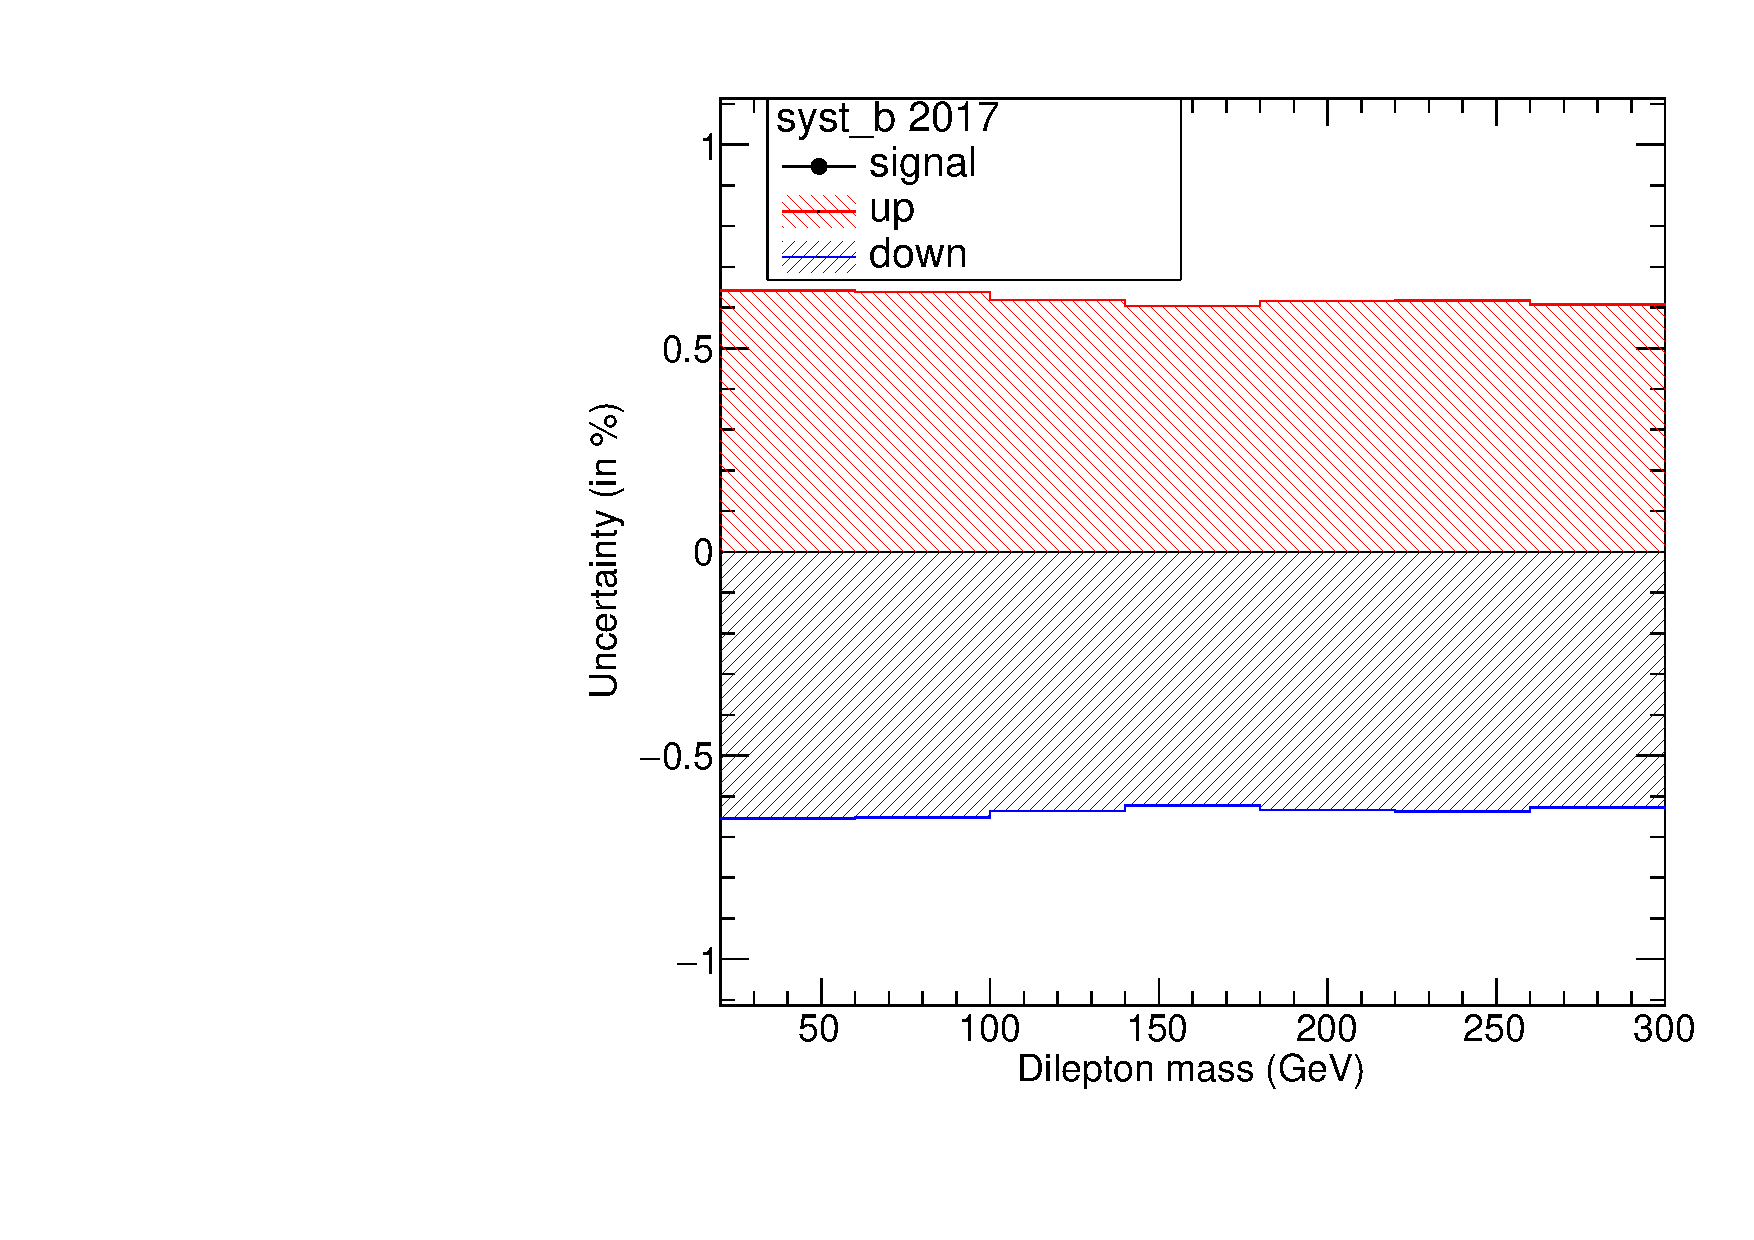
\includegraphics[width=0.8\textwidth]{m_dilep_signal_syst_b_2017.pdf}
        \caption{incertitude sur l'étiquetage des \Pbottom}
        \label{fig:syst_b_2017}
    \end{center}
    \end{subfigure}
        \hspace{0.4cm}
    \begin{subfigure}[b]{0.5\textwidth}
    \begin{center}  
        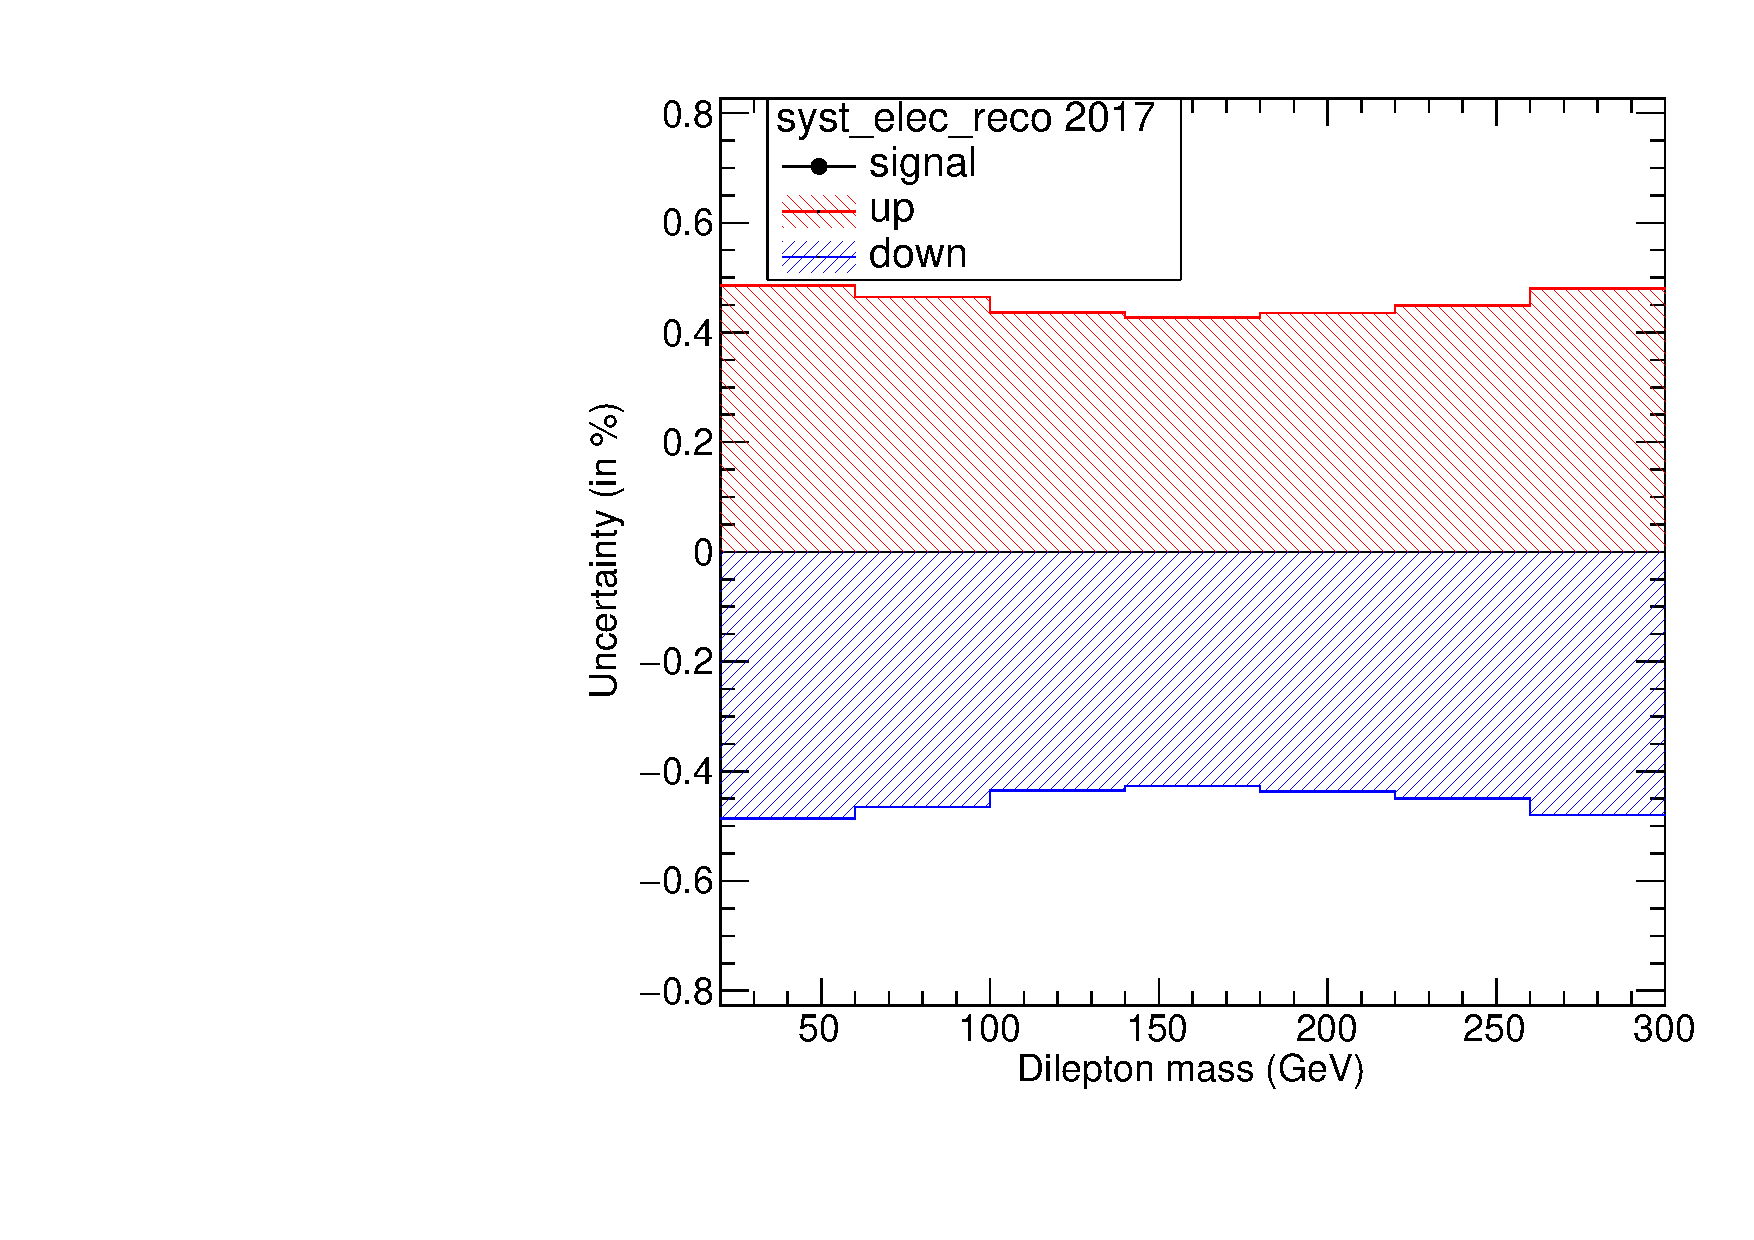
\includegraphics[width=0.8\textwidth]{m_dilep_signal_syst_elec_reco_2017.pdf}
        \caption{incertitude sur la reconstruction des \Pe}
        \label{fig:elec_reco_2017}
    \end{center}
    \end{subfigure}
    \vspace{0.5cm}
    
    \begin{subfigure}[b]{0.5\textwidth}
    \begin{center}
        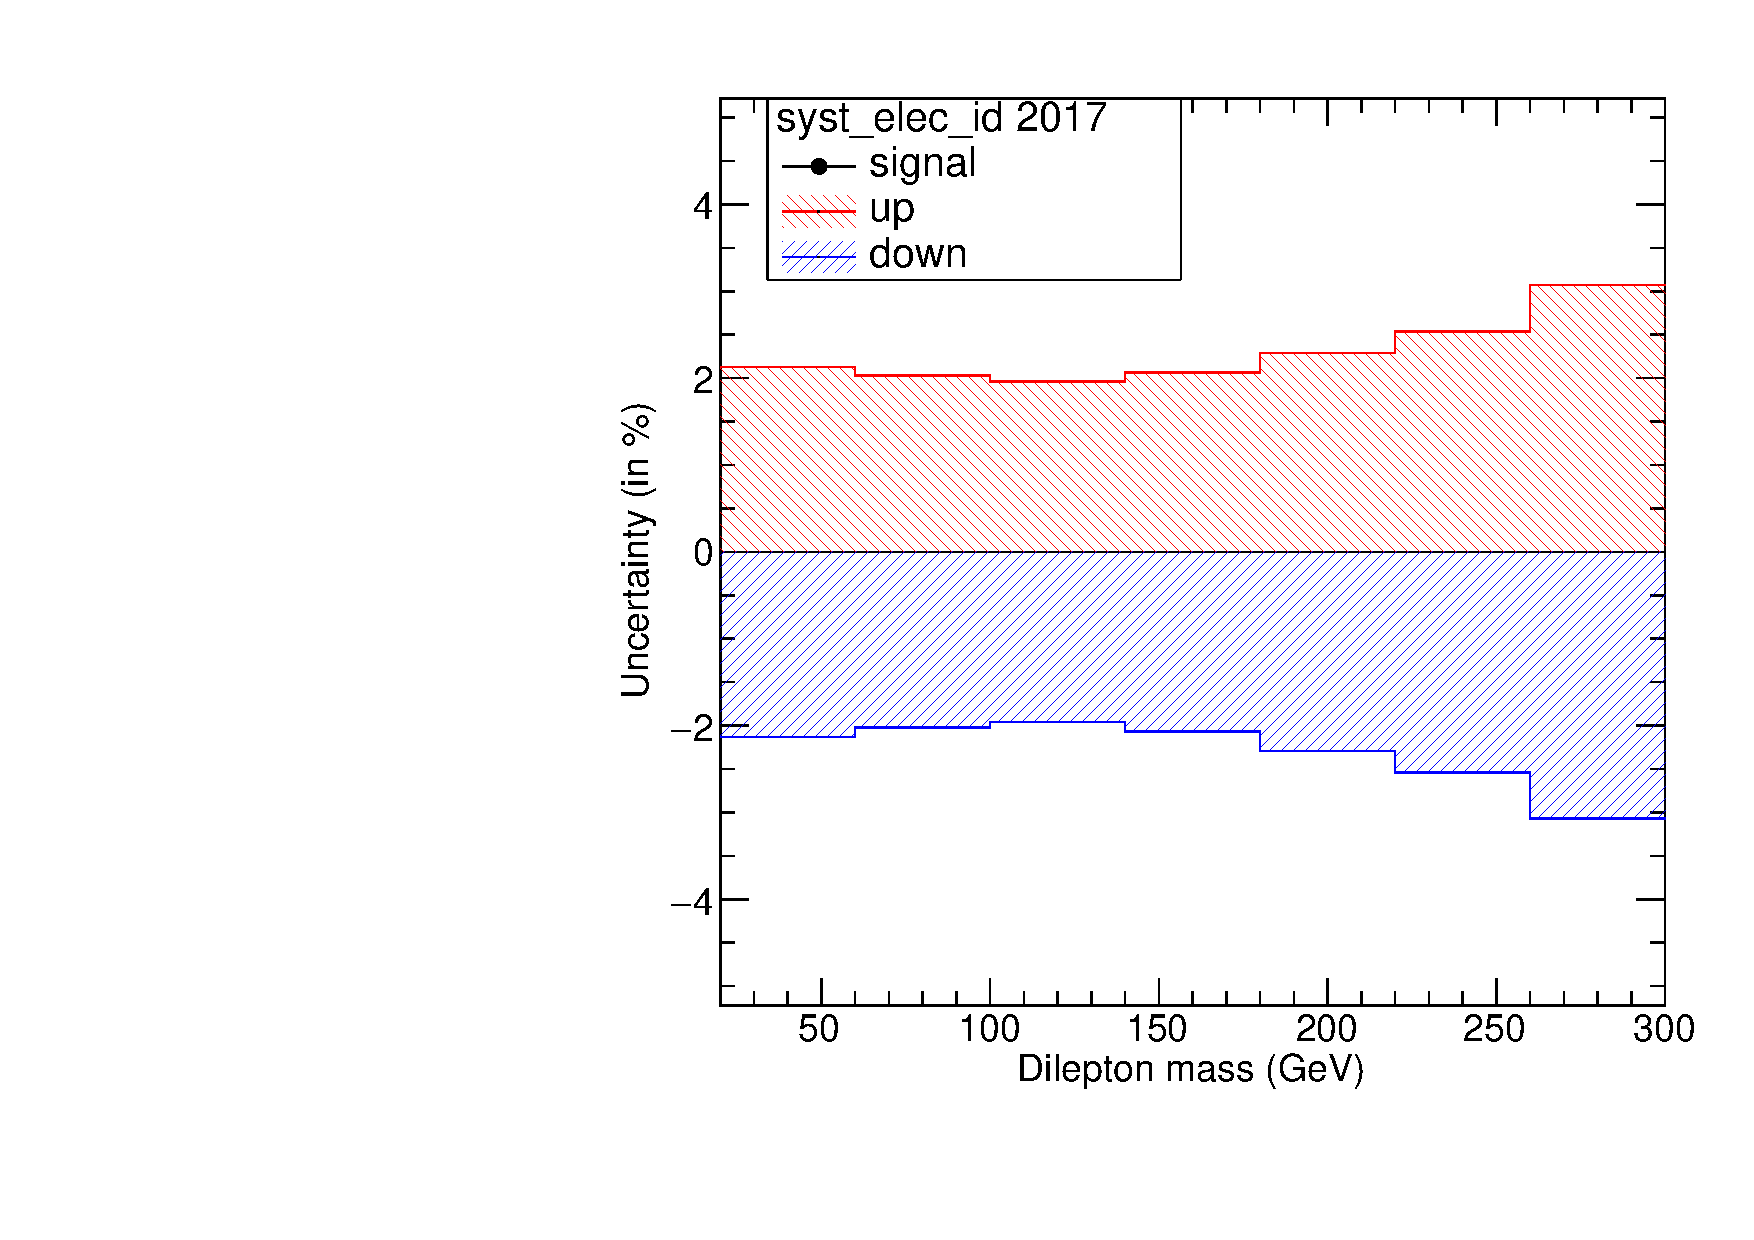
\includegraphics[width=0.8\textwidth]{m_dilep_signal_syst_elec_id_2017.pdf}
        \caption{incertitude sur l'identification des \Pe}
        \label{fig:elec_id_2017}
    \end{center}
    \end{subfigure}
    \hspace{0.4cm}
    \begin{subfigure}[b]{0.5\textwidth}
    \begin{center}
        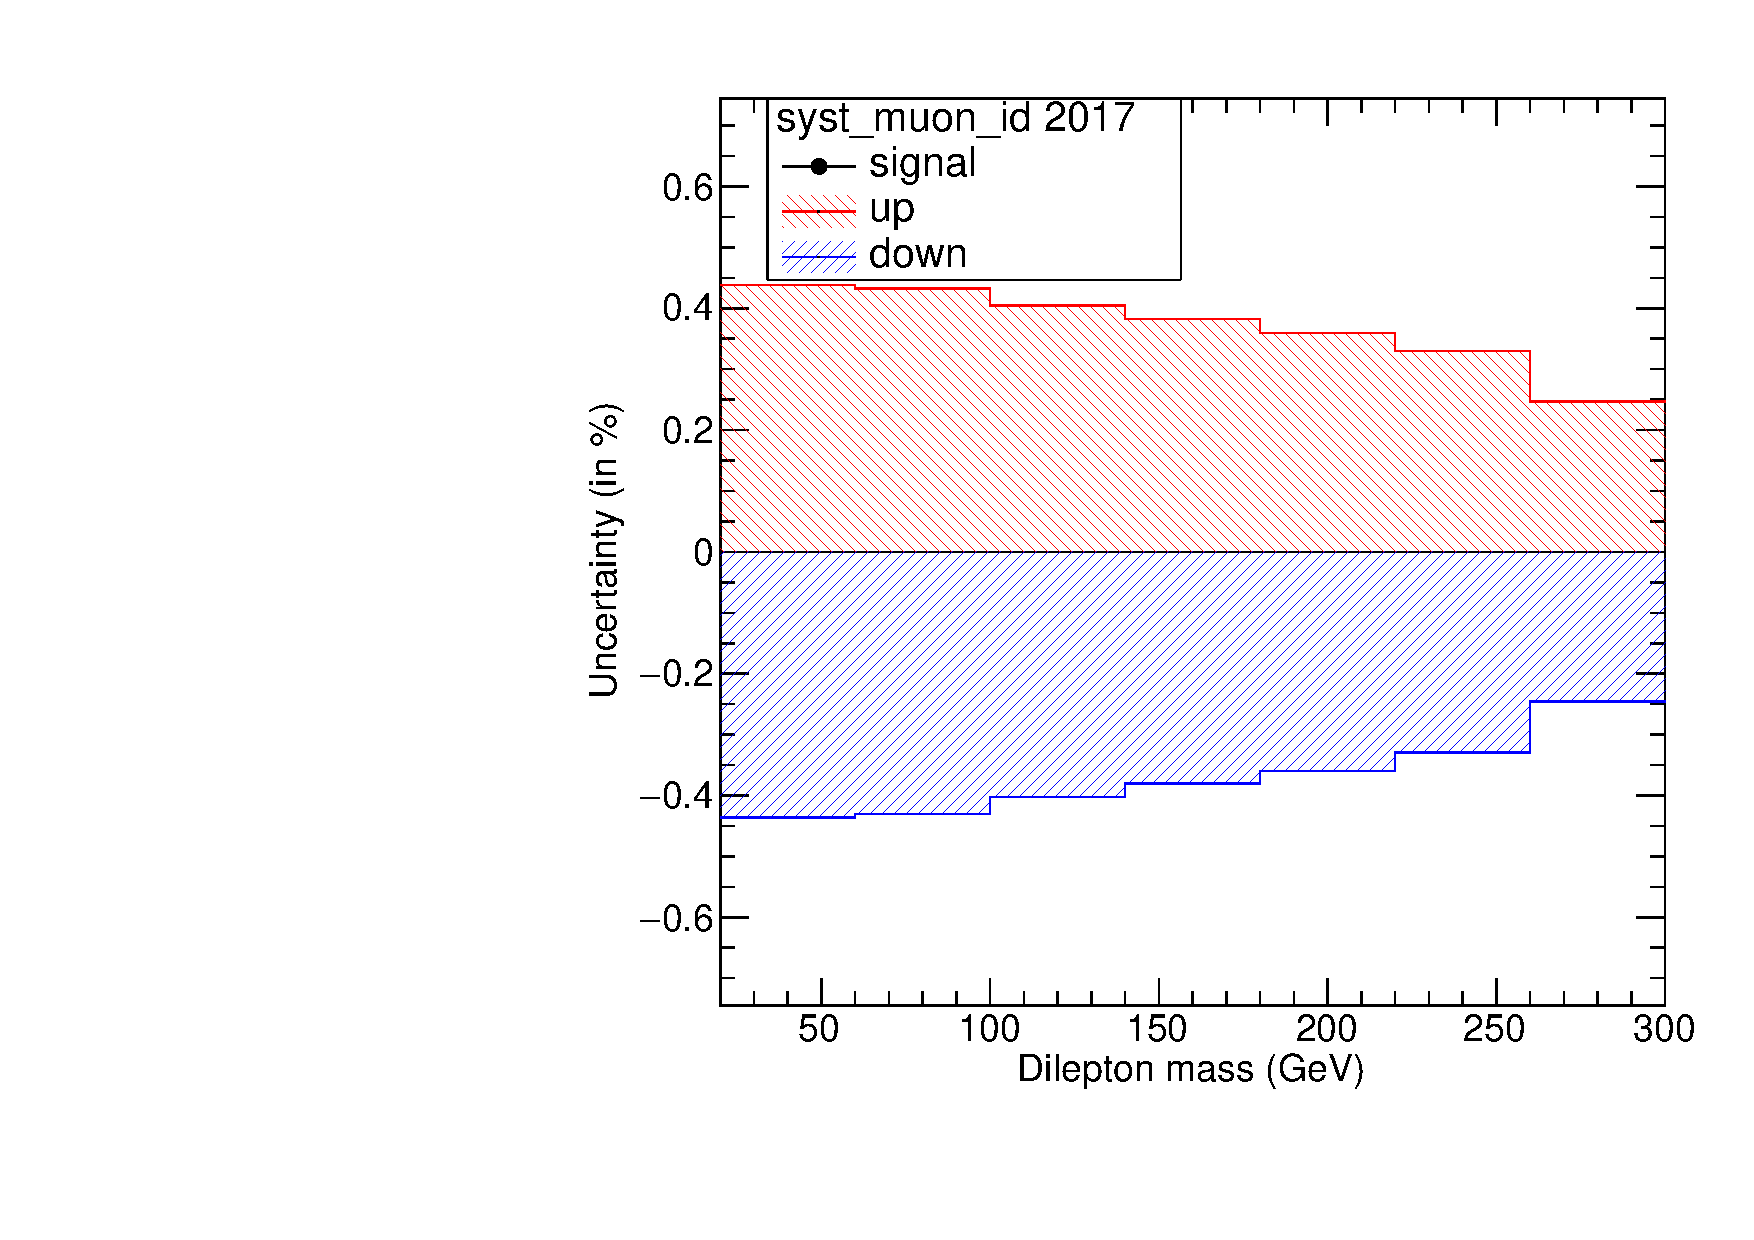
\includegraphics[width=0.8\textwidth]{m_dilep_signal_syst_muon_id_2017.pdf}
        \caption{incertitude sur l'identification des \Pmu}
        \label{fig:muon_id_2017}
    \end{center}
    \end{subfigure}
    \caption{Tracé des incertitudes systématiques pour l'année 2017 avec   (\subref{fig:syst_b_2017}) étiquetage des \Pbottom, (\subref{fig:elec_reco_2017}) reconstruction des électrons, (\subref{fig:elec_id_2017}) identification des électrons et (\subref{fig:muon_id_2017}) identification des muons sur la masse dilepton de l'échantillon Monte-Carlo \ttbar. Chaque histogramme présente des incertitudes relatives.}
\end{figure}


\begin{table}
\centering
\resizebox{0.8\textwidth}{!}{
    \begin{tabular}{cc@{\hspace{2em}}c}
        \noalign{\smallskip}\hline\noalign{\smallskip}
        Source & Type & Valeurs  \\
        \hfill
        & & 2016 $\qquad$ 2017 \\
        \noalign{\smallskip}
        \hline \hline
        \noalign{\smallskip}
        Luminosité (indépendante du temps) & Norme &\SI{1.27}{\%}  $\quad$ \SI{1.67}{\%}  \\
         \Ptop{}\APtop (Modèle Standard) & Norme & \SI{10}{\%} \\
         \Ptop{}\Ptop{}$X$  & Norme & \SI{20}{\%} \\
         \Ptop solitaire & Norme & \SI{30}{\%} \\
         Dibosons & Norme & \SI{30}{\%} \\
         \PWpm{}+ jets & Norme & \SI{30}{\%} \\
         Drell-Yan & Norme & \SI{20}{\%} \\
         \noalign{\smallskip}\hline\noalign{\smallskip}
         Pondération du \pt du quark \Ptop & Forme &  $\pm 1\sigma(\eta,\pt)$\\
         Identification des électrons & Forme & $\pm 1\sigma(\eta,\pt)$\\ 
         Reconstruction des électrons & Forme & $\pm 1\sigma(\eta,\pt)$ \\
         Identification des muons & Forme & $\pm 1\sigma(\eta,\pt)$ \\
         Isolation des muons & Forme &  $\pm 1\sigma(\eta,\pt)$ \\
         Étiquetage du \Pbottom & Forme & $\pm 1\sigma(\eta,\pt)$ \\
         Empilement & Forme & $\pm 1\sigma(\eta,\pt)$ \\
      \noalign{\smallskip}\hline\noalign{\smallskip}
        Correction en énergie des jets & Forme & $\pm 1\sigma(\eta,\pt)$ \\
        Paramètre hdamp & Forme & $\pm 1\sigma(\eta,\pt)$ \\
        Évènement sous-jacent & Forme & $\pm 1\sigma(\eta,\pt)$ \\
        Masse du quark \Ptop & Forme & $\pm 1\sigma(\eta,\pt)$ \\
        Statistiques des Monte-Carlo &  & \\
        \noalign{\smallskip}
        \hline \\
        \multicolumn{3}{c}{Dépendante du temps}\\
        \hline
        \noalign{\smallskip}
        Stabilité de la luminosité & Forme & $\pm 1\sigma(t)$ \\  
        Linéarité de la luminosité & Forme & $\pm 1\sigma(t)$ \\
        Déclenchement \Pe{}\Pmu  & Forme & $\pm 1\sigma(t)$ \\
       \noalign{\smallskip}\hline\noalign{\smallskip} 
    \end{tabular}
}
    \caption{Incertitudes systématiques incluses dans l'ajustement}
    \label{tab:systematics}
\end{table}

\section{Extraction du signal}\label{sec:final}

Comme dans le cas de notre travail phénoménologique (chapitre \ref{chap:chap2}), les résultats temporaires de cette analyse sont obtenus dans les conditions d'un test Asimov. Ce test définit une expérience idéale où le signal est le Modèle Standard seul, donc $c_{\mu\nu} = 0$ par définition. 

Un tel test est demandé par la collaboration CMS pour pouvoir construire une analyse en aveugle. La levée de cette procédure d'"aveuglement" (en anglais \emph{unblinding}) est accordée par la collaboration CMS après validation de l'analyse. Une telle procédure étant longue (parfois plusieurs mois), l'\emph{unblinding} n'a pu être accordé au moment de la rédaction de ce mémoire. Les résultats présentés seront donc systématiquement en contexte de test Asimov.

\subsection{Mesure différentielle en fonction du temps }

Une première étape avant d'effectuer la mesure des $c_{\mu\nu}$ est l'ajustement au cours du temps sidéral de la masse dilepton. Le but, lorsqu'on effectuera l'analyse dans les données, est de pouvoir observer la variation du nombre d'évènements \ttbar en fonction du temps sidéral.  Dans cette mesure, on mesure l'intensité du signal $\mu$ défini comme le rapport du nombre d'évènements du processus \ttbar des données observées sur le  nombre d'évènements \ttbar prédit par le Modèle Standard : 
\begin{equation}
    \mu = \frac{N_\textrm{{\ttbar} observé}}{N_\textrm{{\ttbar} Modèle Standard}}
\end{equation}
L'ajustement est fait en fonction des heures sidérales. 
Les incertitudes systématiques, à la différence des $\mu$, sont toutes corrélées entre les bins de temps. 

\begin{figure}
    \begin{subfigure}[b]{0.45\textwidth}
    \begin{center}
        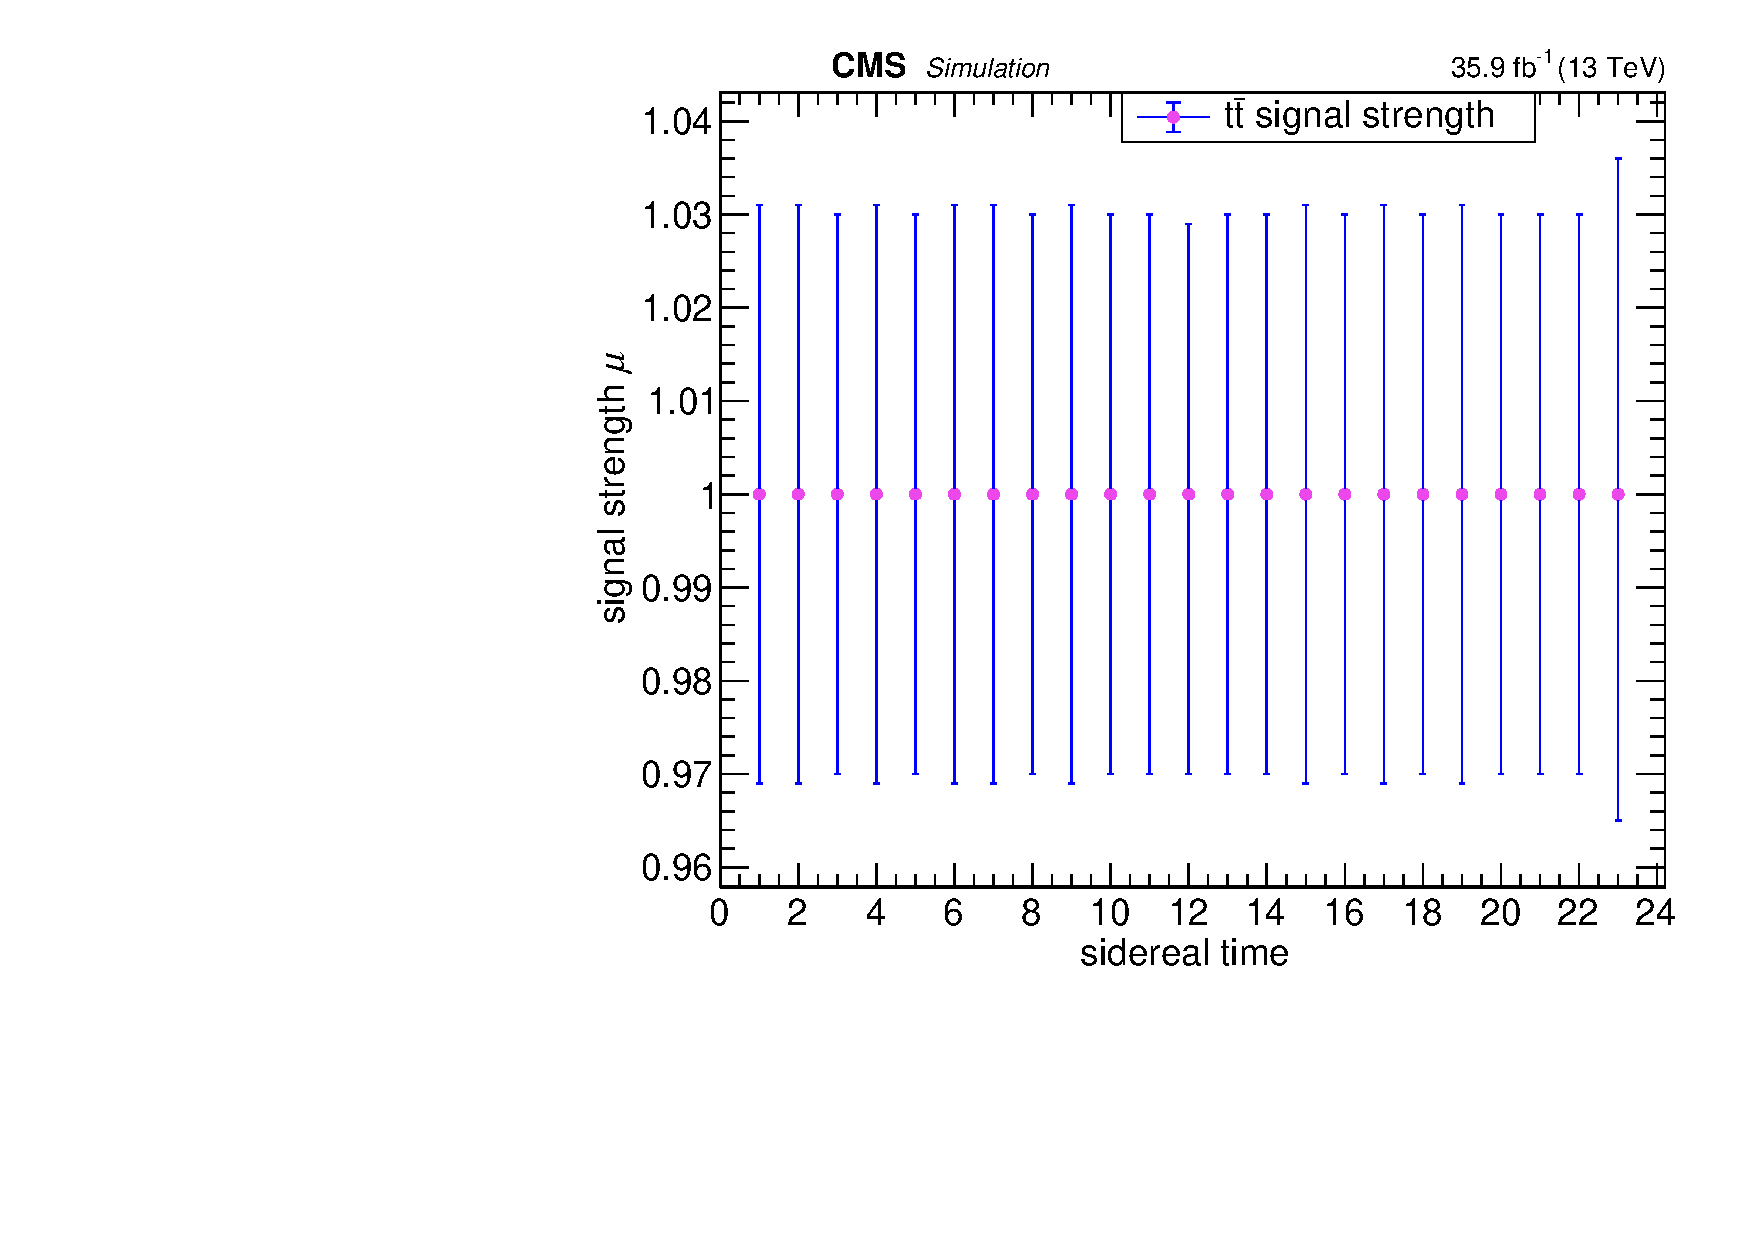
\includegraphics[width=0.8\textwidth]{differential_time_2016.pdf}
        \caption{2016}
        \label{fig:timedeif_2016}
    \end{center}
    \end{subfigure}
    \hspace{0.2cm}
    \begin{subfigure}[b]{0.45\textwidth}
    \begin{center}
        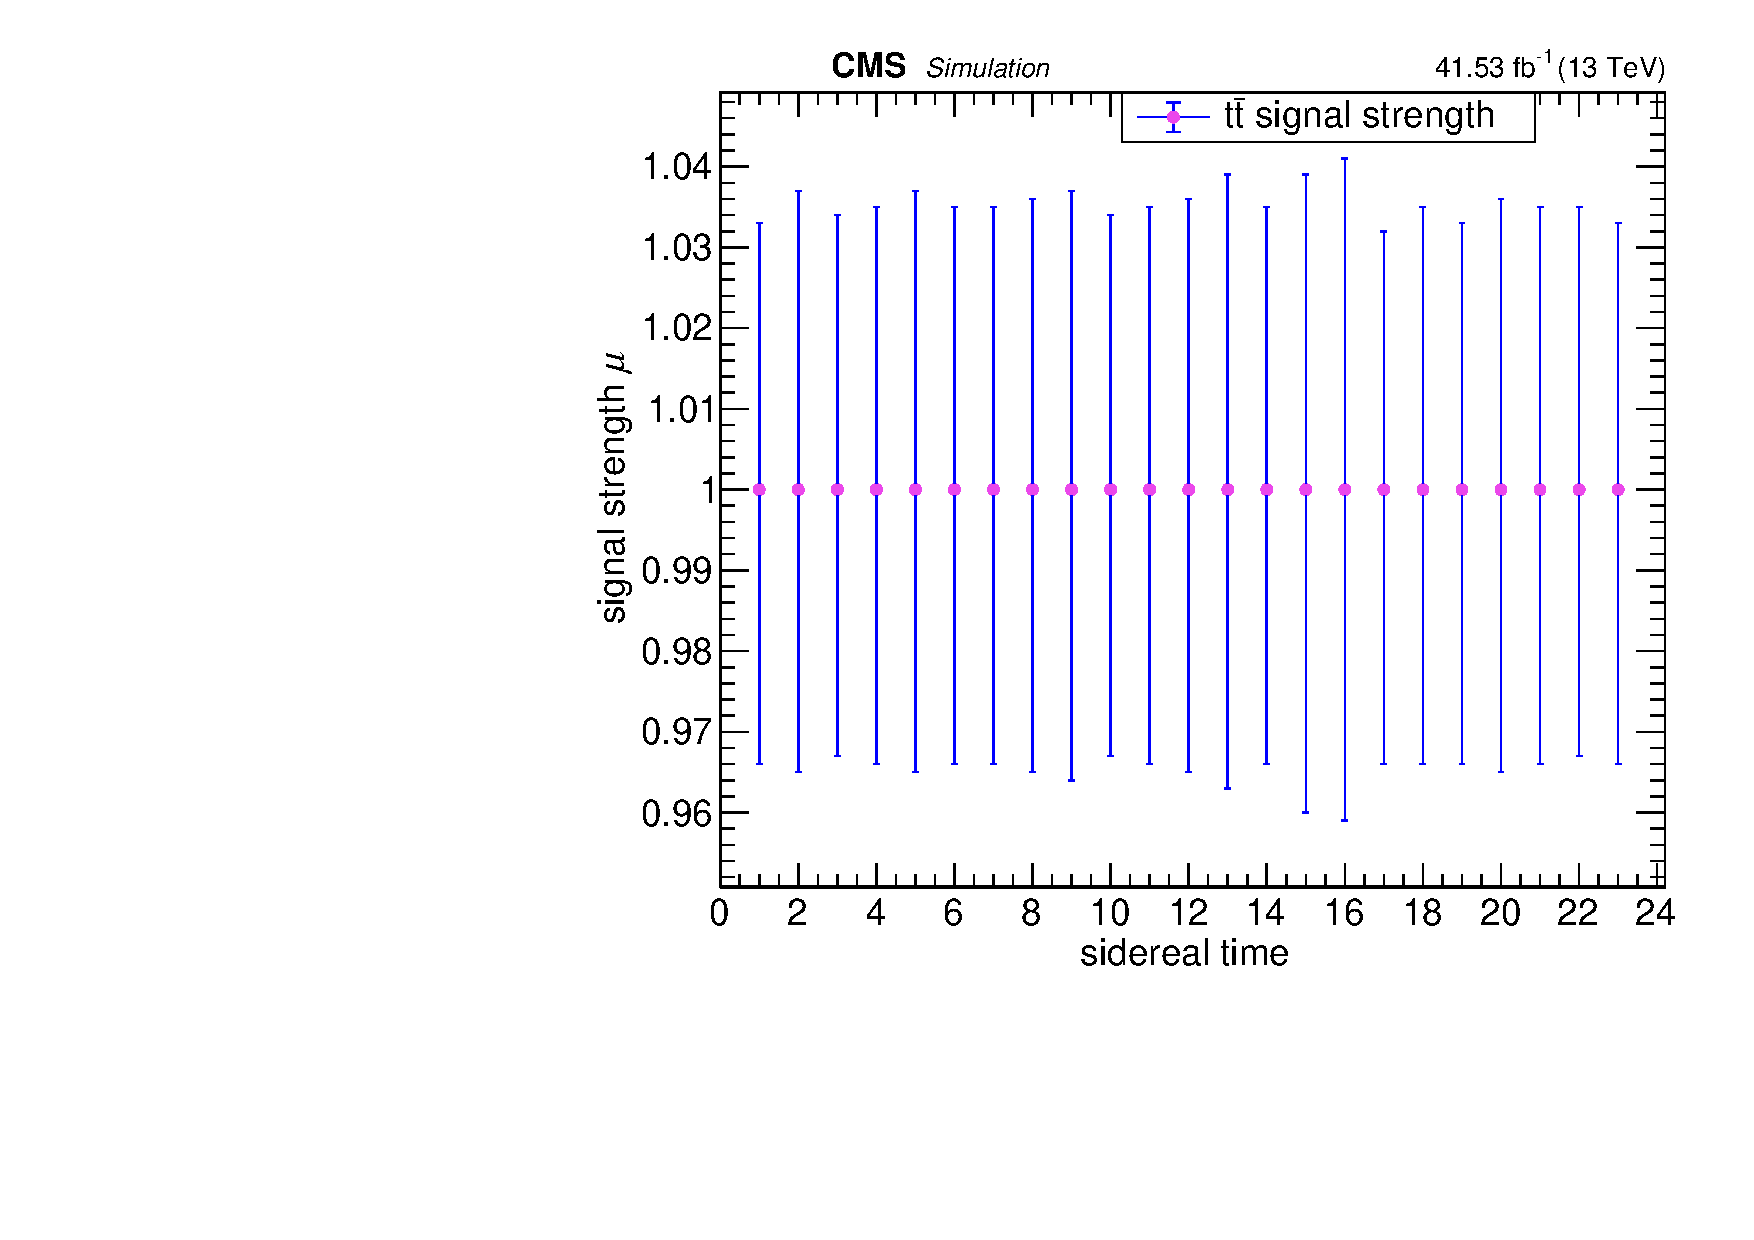
\includegraphics[width=0.8\textwidth]{differential_time_2017.pdf}
        \caption{2017}
        \label{fig:timedeif_2017}
    \end{center}
    \end{subfigure}
    \caption{Mesure différentielle de l'intensité du signal $\mu$ de la masse dilepton au cours du temps sidéral pour l'année (\subref{fig:timedeif_2016}) 2016 et (\subref{fig:timedeif_2017}) 2017, dans la simulation (lot de données Asimov)}
    \label{fig:timediff}
\end{figure}


Un tracé de cette mesure différentielle pour la masse dilepton est donnée en figure \figurename{\ref{fig:timediff}}. Les corrections temporelles dues au déclencheur \Pe{}\Pmu et aux mesures de luminosité montrent une différence de l'erreur sur $\mu$ au cours du temps, qui s'explique par les valeurs des tableaux \tablename{\ref{tab:diff2016}} pour 2016 et \tablename{\ref{tab:diff2017}} pour 2017. 
\begin{table}
\begin{center}
\resizebox{\textwidth}{!}{
\begin{tabular}{c|*{12}{c}}
\noalign{\smallskip}\hline\noalign{\smallskip} 
Heure sidérale &1&2&3&4&5&6&7&8&9&10&11&12 \\
        \noalign{\smallskip}
        \hline \hline
        \noalign{\smallskip}
Incertitude $\uparrow$ &0.031&0.031&0.03&0.031&0.03&0.031&0.031&0.03&0.031&0.03&0.03&0.029\\
Incertitude $\downarrow$ &0.031&0.031&0.03&0.031&0.03&0.031&0.031&0.03&0.031&0.03&0.03&0.03\\
\noalign{\smallskip}\hline\noalign{\smallskip} 
\noalign{\smallskip}\hline\noalign{\smallskip} 
&13&14&15&16&17&18&19&20&21&22&23&24 \\
        \noalign{\smallskip}
        \hline \hline
        \noalign{\smallskip}
Incertitude $\uparrow$ &0.03&0.03&0.031&0.03&0.031&0.03&0.031&0.03&0.03&0.03&0.036&0.03\\
Incertitude $\downarrow$ &0.03&0.03&0.031&0.03&0.031&0.03&0.031&0.03&0.03&0.03&0.035&0.03\\
       \noalign{\smallskip}\hline\noalign{\smallskip} 
\end{tabular}
}
\caption{Valeur des incertitudes sur la mesure différentielle de l'intensité du signal $\mu$ en 24 heures sidérales pour l'année 2016 en test Asimov.}
\label{tab:diff2016}
\end{center}
\end{table}

\begin{table}
\begin{center}
\resizebox{\textwidth}{!}{
\begin{tabular}{c|*{12}{c}}
\noalign{\smallskip}\hline\noalign{\smallskip} 
Heure sidérale &1&2&3&4&5&6&7&8&9&10&11&12 \\
        \noalign{\smallskip}
        \hline \hline
        \noalign{\smallskip}
Incertitude $\uparrow$&0.033&0.037&0.034&0.035&0.037&0.035&0.035&0.036&0.037&0.034&0.035&0.036\\
Incertitude $\downarrow$ &0.034&0.035&0.033&0.034&0.035&0.034&0.034&0.035&0.036&0.033&0.034&0.035\\
\noalign{\smallskip}\hline\noalign{\smallskip} 
\noalign{\smallskip}\hline\noalign{\smallskip} 
&13&14&15&16&17&18&19&20&21&22&23&24 \\
        \noalign{\smallskip}
        \hline \hline
        \noalign{\smallskip}
Incertitude $\uparrow$ &0.039&0.035&0.039&0.041&0.032&0.035&0.033&0.036&0.035&0.035&0.033&0.037\\
Incertitude $\downarrow$ &0.037&0.034&0.04&0.041&0.034&0.034&0.034&0.035&0.034&0.033&0.034&0.035\\
       \noalign{\smallskip}\hline\noalign{\smallskip} 
\end{tabular}
}
\caption{Valeur des incertitudes sur la mesure différentielle de l'intensité du signal $\mu$ en 24 heures sidérales pour l'année 2017 en test Asimov.}
\label{tab:diff2017}
\end{center}
\end{table}

Avec une mesure inclusive, on a une estimation moyenne de  $\mu^\textrm{2016} = \num{1}^{+0.029}_{-0.028} \textrm{(stat+syst)}$ et $\mu^\textrm{2017} = \num{1}^{+0.029}_{-0.028} \textrm{(stat+syst)}$. 

\subsection{Mesure des paramètres $c_{\mu\nu}$ dans le SME}

L'étape finale de cette analyse est la mesure des coefficients de Wilson $c_{\mu\nu}$. Pour rappel ces coefficients sont présentés dans la section \ref{sec:TheSME} du chapitre \ref{chap:chap1} et définissent l'amplitude d'oscillation de la section efficace du processus \ttbar par l'équation :
\begin{equation*}
 \sigma_\textrm{SME}  = (1+ f(t)) \sigma_\textrm{SM}
\end{equation*}
avec $f(t)$ la fonction d'oscillation. Le test Asimov impliquera une mesure dans laquelle les fausses données issues de la simulation n'incluent pas de signal, donc $c_{\mu\nu} = 0$, par définition. Le but de cette étude est donc d'estimer l'incertitude attendue $\Delta c_{\mu\nu}$ sur la mesure des différents coefficients de Wilson.
\newline

Cette mesure évalue par ajustement la valeur de l'intensité du signal $\mu$ simultanément sur tous les bins de temps. En utilisant la densité de probabilité de Poisson $\rho$ présentée dans l'équation \eqref{Poisson}, on a dans le cadre de l'analyse :
\begin{equation}
    \rho = \mu \mathcal{S} + \mathcal{B}
\end{equation} 
où $\mathcal{S}$ est l'histogramme de la masse dilepton du SME et $\mathcal{B}$ l'histogramme de la masse dilepton du Modèle Standard. Par rapport au signal du Modèle Standard l'oscillation générée par le SME implique une densité de probabilité qui peut prendre des valeurs négatives. Le programme de CMS ne pouvant traiter de tels cas nous avons d\^u créer un modèle physique propre à l'analyse. Nous avons construit un modèle de type : 
\begin{equation}
\rho =  \mu \left( \mathcal{S} + \mathcal{B}\right) + \left( 1 - \mu \right) \mathcal{B}
\end{equation}
Ceci permet d'assurer une densité de probabilité positive grâce à l'histogramme $\mathcal{S} + \mathcal{B}$ positif quelque soit $\mu$ entre 0 et 1. 

Comme expliqué dans la section \ref{sec:likelihood}, les coefficients $c_{\mu\nu}$ sont proportionnels au paramètre $\mu$. On aura donc pour extraire la valeur finale des coefficients de Wilson :
\begin{equation}
c_{\mu\nu} = \alpha \mu
\end{equation}
avec $\alpha$ la valeur de l'amplitude de l'oscillation temporelle choisie pour construire le signal théorique à ajuster.
\newline

Avec un test Asimov, l'ajustement par maximum de vraisemblance a été effectué en utilisant comme variable discriminante la masse dilepton pour les années 2016 et 2017. 
Les histogrammes utilisés pour l'extraction du signal sont des histogrammes dans lesquels on a réparti la masse dilepton sur 24 bins représentant pour chacun une heure sidérale. Un exemple de ces histogrammes est présenté dans la figure \figurename{\ref{fig:unrolled}}.

\begin{figure}
    \begin{center}
        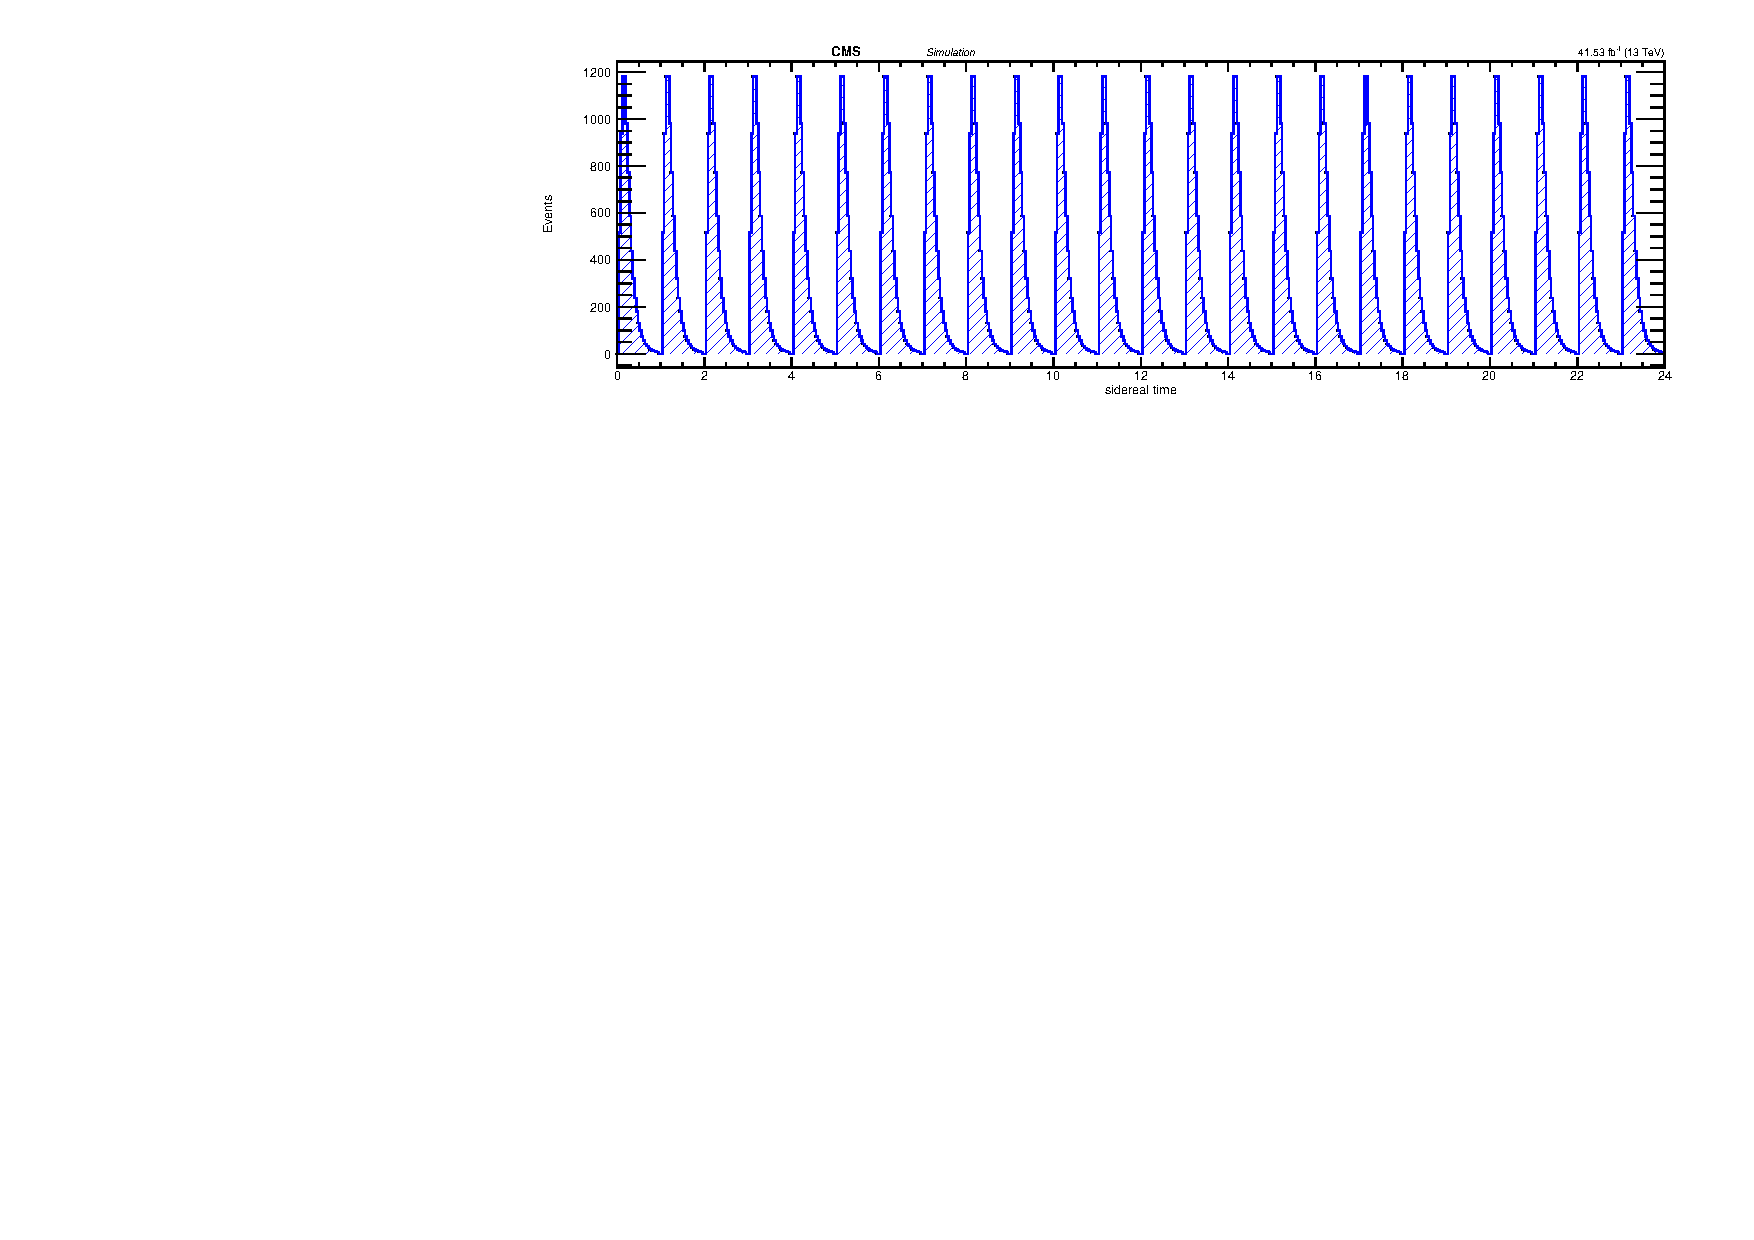
\includegraphics[width=0.32\textwidth]{unrolled.pdf}
        \caption{Histogramme accolé présentant la masse dilepton provenant du processus \ttbar du Modèle Standard pour l'année 2017.}
        \label{fig:unrolled}
    \end{center}
\end{figure}


Le tableau \tablename{\ref{tab:final}} présente ces mesures pour l'ensemble des coefficients de Wilson du SME que nous avons identifié au chapitre \ref{chap:chap1} :  

\begin{table}[H]
\centering
    \resizebox{0.9\textwidth}{!}{
    \begin{tabular}{ccc@{\qquad}|@{\quad}c}
        \hline\noalign{\smallskip}
         Coefficient de Wilson & \multicolumn{2}{c@{\qquad}|@{\quad}}{LHC - Run II} & Étude phénoménologique \cite{Carle_2020}  \\
           &  2016   & 2017& \\
        \noalign{\smallskip}
        \hline \hline
        \noalign{\smallskip}
        $\Delta c_{LXX}$ & $2.51\times 10^{-4}$  & $2.32\times 10^{-4}$&
        $7\times 10^{-4}$ \\
        $\Delta c_{LXY}$ & $2.54\times 10^{-4}$  & $2.32\times 10^{-4}$&
        $7\times 10^{-4}$ \\
        $\Delta c_{LXZ}$ & $0.92\times 10^{-3}$ & $0.85\times 10^{-3}$ &
        $3\times 10^{-3}$\\
        $\Delta c_{LYZ}$ & $0.94\times 10^{-3}$ & $0.86\times 10^{-3}$ &
        $3\times 10^{-3}$\\
        \noalign{\smallskip}\hline\noalign{\smallskip}
        $\Delta c_{RXX}$ & $0.87\times 10^{-3}$  & $0.81\times 10^{-3}$&
         $3\times 10^{-3}$\\
        $\Delta c_{RXY}$ & $0.88\times 10^{-3}$  & $0.81\times 10^{-3}$&
         $3\times 10^{-3}$\\
        $\Delta c_{RXZ}$ & $0.32\times 10^{-2}$ & $0.29\times 10^{-2}$ &
        $1\times 10^{-2}$ \\
        $\Delta c_{RYZ}$ & $0.32\times 10^{-2}$ & $0.29\times 10^{-2}$ &
        $1\times 10^{-2}$ \\
        \noalign{\smallskip}\hline\noalign{\smallskip}
        $\Delta c_{XX}$ & $0.35\times 10^{-3}$  & $0.33\times 10^{-3}$ &
         $1\times 10^{-3}$\\
        $\Delta c_{XY}$ & $0.36\times 10^{-3}$  & $0.33\times 10^{-3}$ &
         $1\times 10^{-3}$\\
        $\Delta c_{XZ}$ & $1.29\times 10^{-3}$ & $1.19\times 10^{-3}$  &
        $4\times 10^{-3}$ \\
        $\Delta c_{YZ}$ & $1.31\times 10^{-3}$ & $1.21\times 10^{-3}$  &
        $4\times 10^{-3}$ \\
        \noalign{\smallskip}\hline\noalign{\smallskip}
        $\Delta d_{XX}$ & $1.95\times 10^{-4}$  & $1.81\times 10^{-4}$ &
        $6\times 10^{-4}$ \\
        $\Delta d_{XY}$ & $1.97\times 10^{-4}$  & $1.81\times 10^{-4}$ &
        $6\times 10^{-4}$ \\
        $\Delta d_{XZ}$ & $0.71\times 10^{-3}$ & $0.66\times 10^{-3}$ &
         $2\times 10^{-3}$\\
        $\Delta d_{YZ}$ & $0.72\times 10^{-3}$ & $0.67\times 10^{-3}$ &
         $2\times 10^{-3}$\\
        \noalign{\smallskip}\hline\vspace{0.1cm}
    \end{tabular}
    }
    \caption{Mesure de la limite des coefficients $c_{\mu\nu}$, avec test Asimov, pour l'année 2016 et 2017. Les prédictions de l'étude phénoménologique présentées dans le chapitre \ref{chap:chap2}, sont aussi données.}
    \label{tab:final}
\end{table}

Le premier constat est l'amélioration de la précision de chaque coefficient par rapport à la précision établie par notre travail phénoménologique présenté au chapitre \ref{chap:chap2}. Les raisons de cette amélioration sont présentées dans la section \ref{discussion} (section Discussion). Avec une étude sur l'année 2018 et une combinaison des précisions, l'erreur sur ces coefficients pourra être améliorée. Confirmant la proposition de l'étude phénoménologique, ce travail de recherche permet de conclure à une augmentation significative de la précision sur les mesures des coefficients de Wilson du SME dans le secteur du quark \Ptop par rapport à la première étude menée par l'expérience D$\emptyset$ \cite{D0}.

\subsection{Impacts des incertitudes systématiques}

Pour pouvoir mettre en évidence l'intégrité de l'ajustement, on étudie l'impact des paramètres de nuisance sur le modificateur d'intensité du signal $\mu$. $\mu$ étant pour rappel, dans cette analyse, proportionnel aux coefficients de Wilson $c_{\mu\nu}$. Dans la suite on parlera de $\mu$ ou des coefficients $c_{\mu\nu}$ sans distinction.
\newline  

L'impact d'un paramètre de nuisance donné $\vartheta$ sur $\mu$ est défini comme le décalage $\Delta \mu$ introduit par un effet de \SI{\pm 1}{\sigma_\vartheta} où $\sigma_\vartheta$ est l'incertitude du paramètre de nuisance après ajustement. Cette mesure permet d'identifier la corrélation entre un paramètre de nuisance et $\mu$, et ainsi de dégager quelle incertitude systématique aura le plus d'impact sur $\mu$.

Les figures \figurename{\ref{fig:impact2016}} et \figurename{\ref{fig:impact2017}} présentent l'impact des différentes incertitudes systématiques sur le coefficient de Wilson $c_{LXX}$ respectivement pour les années 2016 et 2017. La partie gauche de ces graphes montre la fraction
\begin{equation*}
\frac{\hat{\vartheta}-\vartheta_0}{\sigma_\vartheta}
\end{equation*}
où $\vartheta$ est la valeur du paramètre après ajustement, $\vartheta_0$ sa valeur initiale et $\sigma_\vartheta$ l'erreur sur $\vartheta$ après ajustement. Pour un test Asimov, cette fraction est toujours nulle car on impose que le résultat  de l'ajustement donne bien la valeur initiale. Lorsque la valeur de l'incertitude de cette fraction se rapproche de 1, cela s'interprète comme le fait que le paramètre de nuisance en question n'est pas contraint par l'ajustement. 

La partie droite des graphes présente l'impact sur $c_{LXX}$ du décalage du paramètre $\vartheta$ de \SI{\pm 1}{\sigma_\vartheta}. Ainsi on constate que les plus gros impacts sont donnés par les incertitudes systématiques liées à la luminosité plate et à la stabilité de la luminosité.

\newpage

\begin{figure}[H]
    \begin{center}
        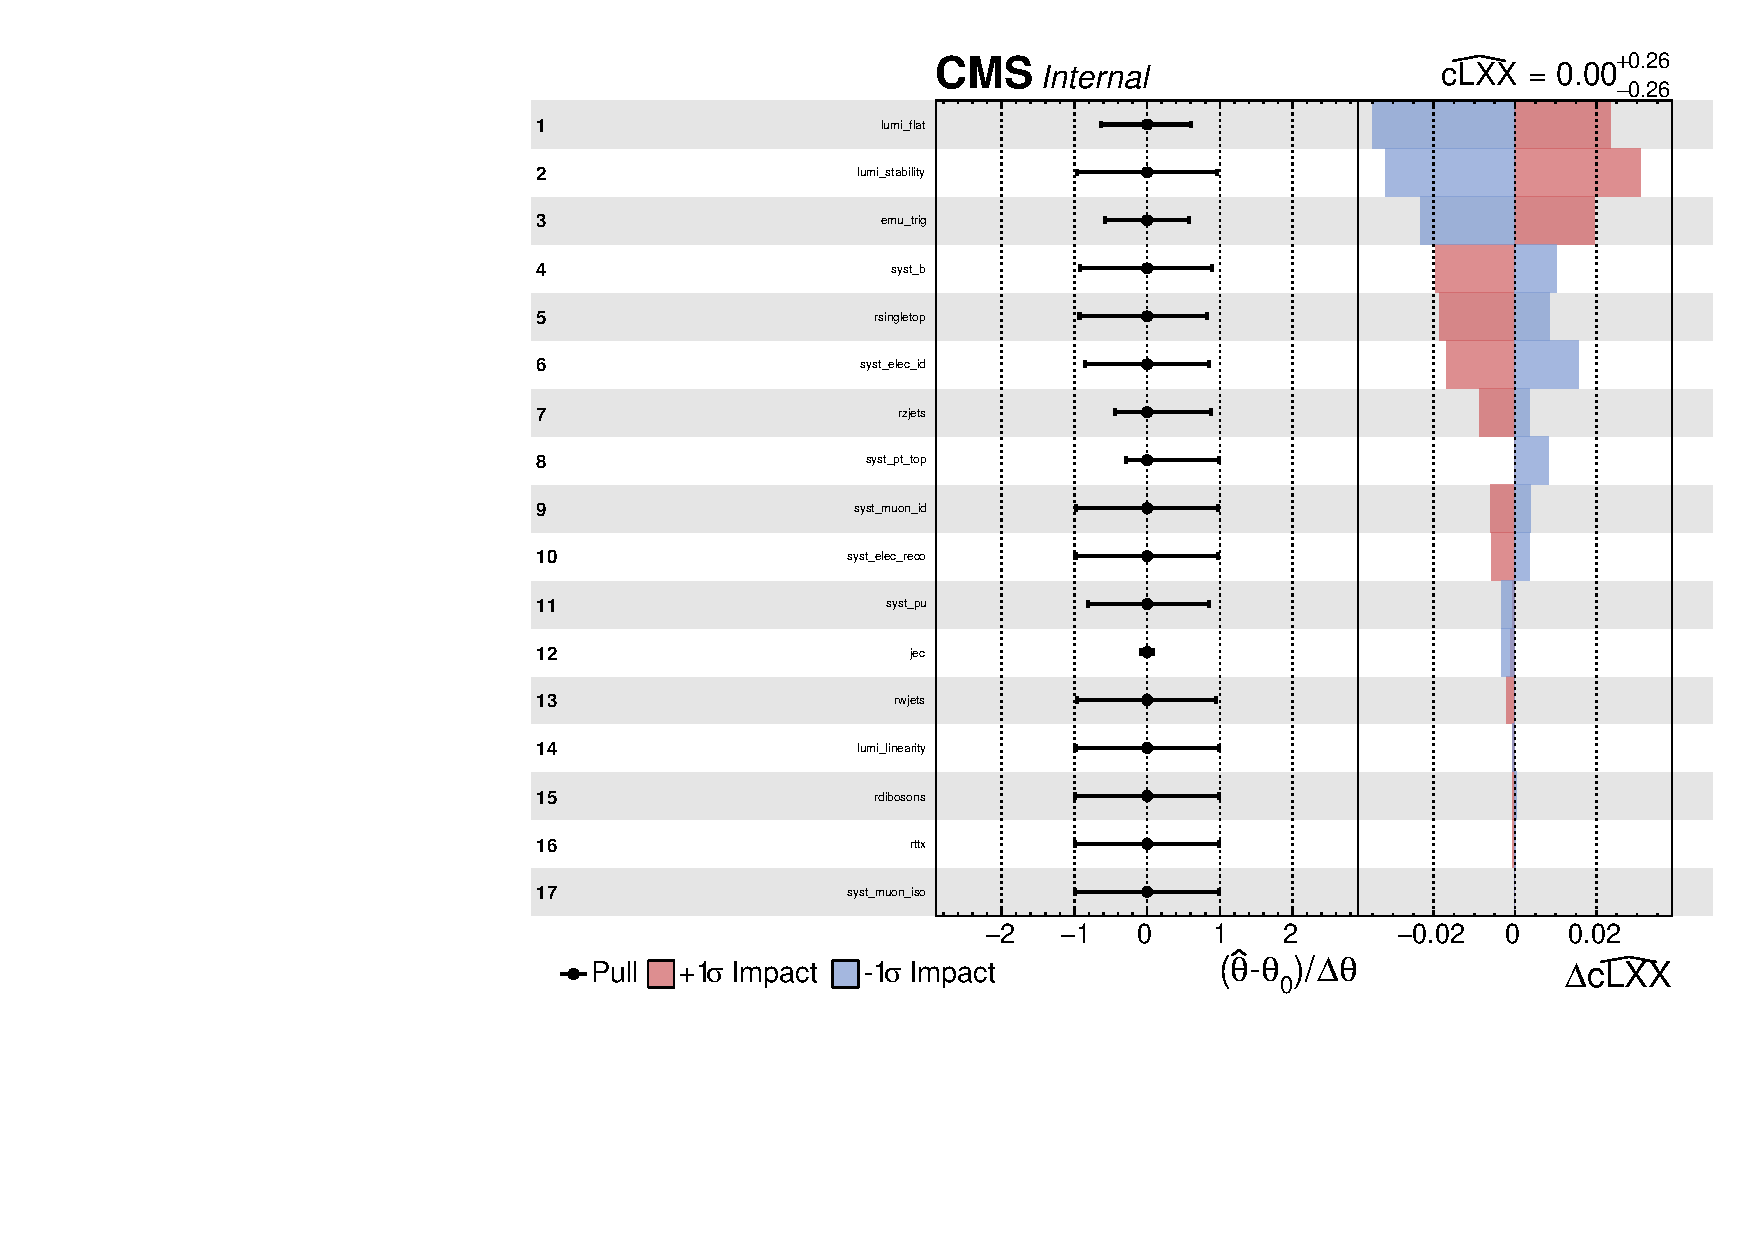
\includegraphics[height=0.35\paperheight]{m_dilep_cLXX_impacts_2016fin.pdf}
        \caption{Graphe d'impact des paramètres de nuisances sur la mesure du coefficient de Wilson $c_{LXX}$ en cas de test Asimov pour l'année 2016. Les valeurs sont à multiplier par un facteur \num{e-3}, autrement dit le graphe indiquant $\Delta c =  \num{2.4e-1}$ signifie le résultat $\Delta c = \num{2.4e-4}$.}
        \label{fig:impact2016}
    \end{center}
\end{figure}

\begin{figure}[H]
    \begin{center}
        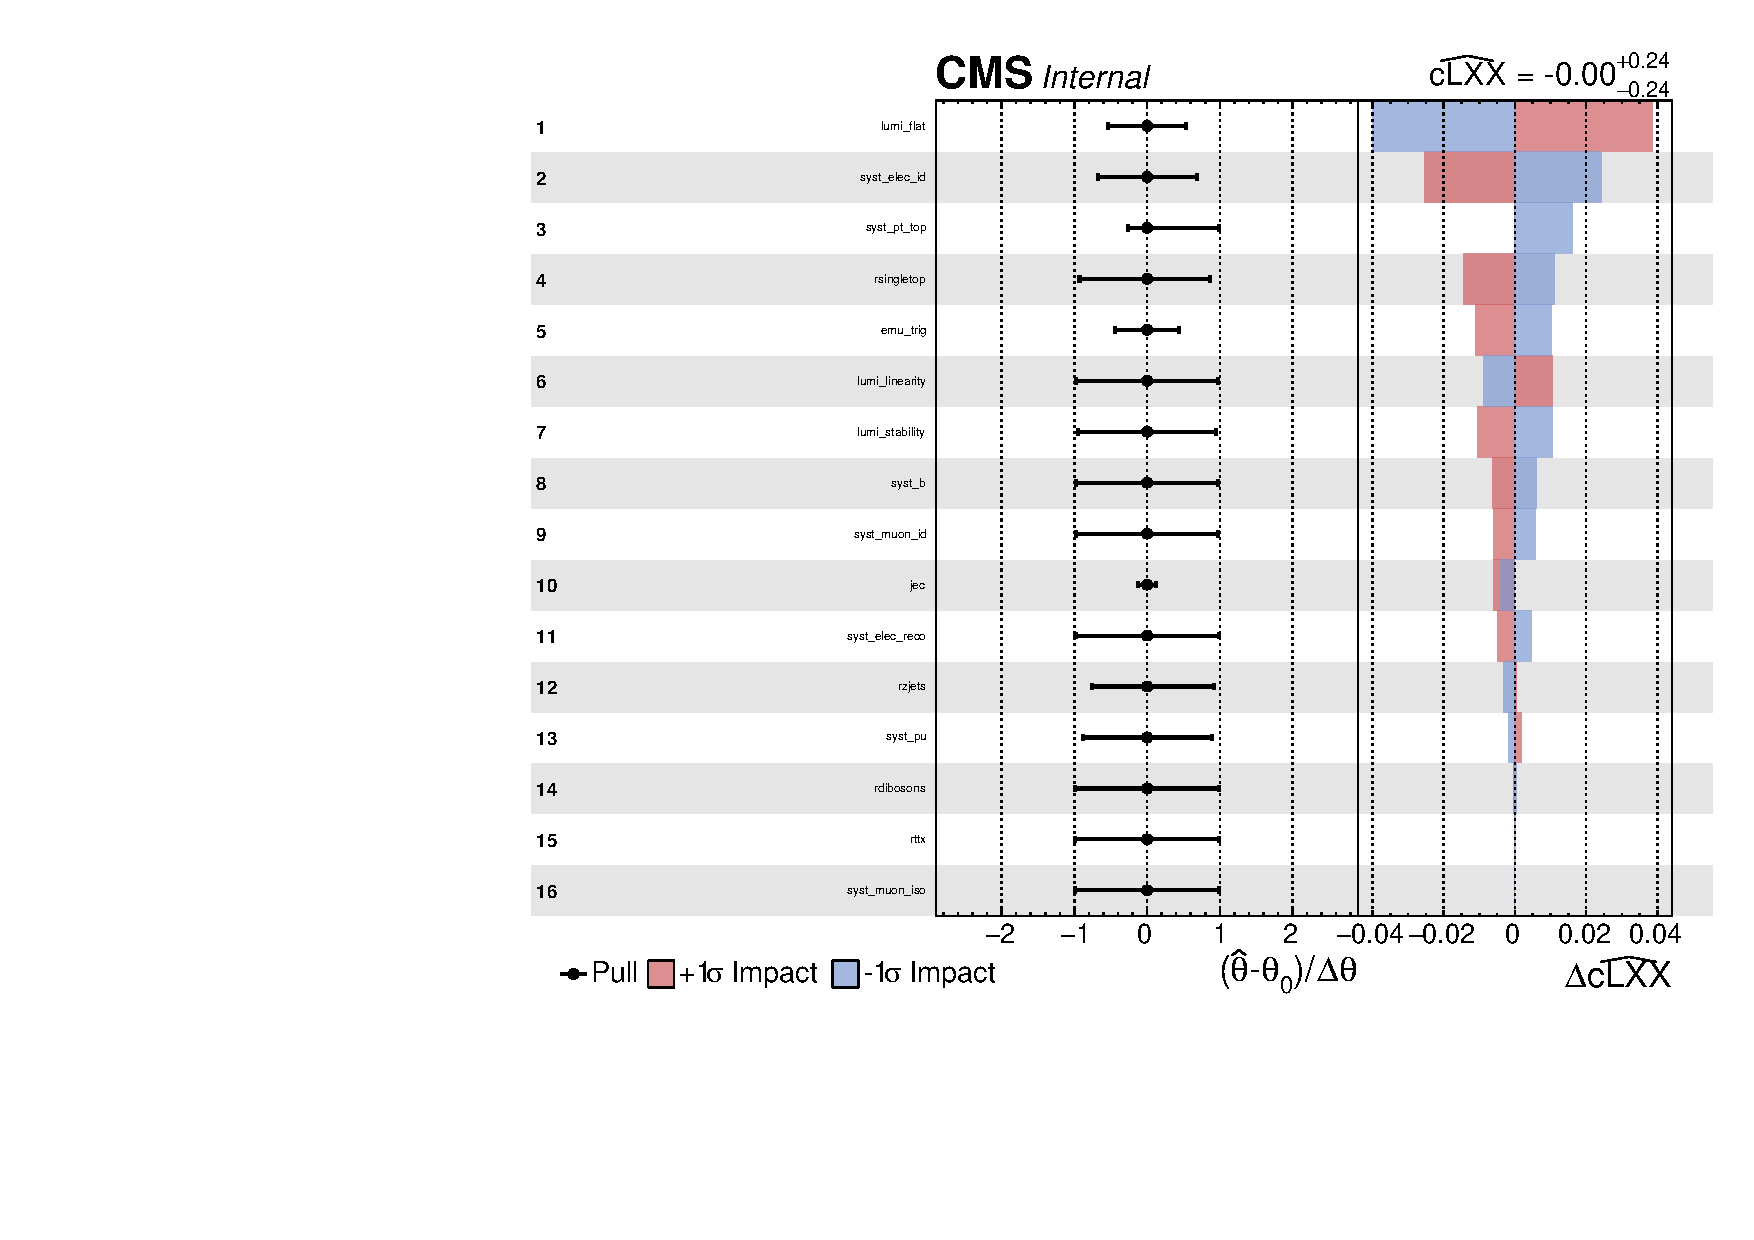
\includegraphics[height=0.35\paperheight]{m_dilep_cLXX_impacts_2017fin.pdf}
        \caption{Graphe d'impact des paramètres de nuisances sur la mesure du coefficient de Wilson $c_{LXX}$ en cas de test Asimov pour l'année 2017. Les valeurs sont à multiplier par un facteur \num{e-3}, autrement dit le graphe indiquant $\Delta c =  \num{2.4e-1}$ signifie le résultat $\Delta c = \num{2.4e-4}$.}
        \label{fig:impact2017}
    \end{center}
\end{figure}

\newpage

\subsection{Discussion}\label{discussion}

Cette étude statistique a permis d'établir la sensibilité sur la mesure des coefficients de Wilson $c_{\mu\nu}$. On peut noter une meilleure précision sur nos  mesures que celle que nous avons établie lors de l'étude phénoménologique. En effet par exemple pour le coefficient $c_{LXX}$ notre prédiction est de $\Delta c_{LXX} = \num{7e-4}$ à \SI{150}{\femto\barn^{-1}} or on obtient respectivement pour 2016 (\SI{39.10}{\femto\barn^{-1}}) et 2017 (\SI{41.53}{\femto\barn^{-1}}) les précisions $\Delta c_{LXX} = \num{2.51e-4}$ et $\Delta c_{LXX} = \num{2.32e-4}$. 

Ce gain de précision est d\^u à plusieurs facteurs. Le premier, est le fait que pour notre étude de faisabilité nous avons utilisé une méthode statistique de $\chi^2$ contre une méthode de maximum de vraisemblance plus puissante en vertu du théorème de Neyman-Pearson. De plus, l'étude des incertitudes systématiques est plus fine pour l'analyse avec des incertitudes de diverses natures (formes, norme) optimisées contre des systématiques de nature norme majorée. Mais la différence majeure provient du fait que l'étude phénoménologique fut établie avec le nombre d'évènements comme variable discriminante. En effet, pour l'analyse avec les données de CMS, la masse dilepton a été utilisée. Ainsi une contrainte provenant de la forme de la distribution est ajoutée. 

Fort de cette étude, la prochaine étape est la mesure sur les données après validation et l'autorisation de la collaboration CMS. Ainsi l'augmentation annoncée de la précision sur la mesure des $c_{\mu\nu}$ par rapport à celle réalisée par l'expérience à D$\emptyset$ pourra être validée, et les données apporteront une réponse quant à la présence ou non d'un signal. 

\end{fmffile}